%--------------------------------------------------------------
% thesis.tex 
%--------------------------------------------------------------
% Corso di Laurea in Informatica 
% http://if.dsi.unifi.it/
% @Facolt\`a di Scienze Matematiche, Fisiche e Naturali
% @Universit\`a degli Studi di Firenze
%--------------------------------------------------------------
% - template for the main file of Informatica@Unifi Thesis 
% - based on Classic Thesis Style Copyright (C) 2008 
%   Andr\'e Miede http://www.miede.de   
%--------------------------------------------------------------
\documentclass[twoside,openright,titlepage,fleqn,
	headinclude,11pt,a4paper,BCOR5mm,footinclude
	]{scrbook}
%--------------------------------------------------------------
\newcommand{\myTitle}{Model checking come supporto per le scelte di sistemi adattivi\xspace}
% use the right myDegree option
\newcommand{\myDegree}{Corso di Laurea Magistrale in Informatica\xspace}
%\newcommand{\myDegree}{
	%Corso di Laurea Specialistica in Scienze e Tecnologie 
	%dell'Informazione\xspace}
\newcommand{\myName}{Marco Tinacci\xspace}
\newcommand{\myProf}{Rocco De Nicola\xspace}
\newcommand{\myOtherProf}{Michele Loreti\xspace}
%\newcommand{\mySupervisor}{Nome Cognome\xspace}
\newcommand{\myFaculty}{
	Facolt\`a di Scienze Matematiche, Fisiche e Naturali\xspace}
\newcommand{\myDepartment}{
	Dipartimento di Sistemi e Informatica\xspace}
\newcommand{\myUni}{\protect{
	Universit\`a degli Studi di Firenze}\xspace}
\newcommand{\myLocation}{Firenze\xspace}
\newcommand{\myTime}{Anno Accademico 2012-2013\xspace}
\newcommand{\myVersion}{Version 0.1\xspace}

%--------------------------------------------------------------
% Theme's packages
%--------------------------------------------------------------
%\usepackage[latin1]{inputenc} 
\usepackage[T1]{fontenc} 
\usepackage[square,numbers]{natbib}
%\usepackage[fleqn]{amsmath}
%--------------------------------------------------------------
\usepackage{dia-classicthesis-ldpkg} 
%--------------------------------------------------------------
% Options for classicthesis.sty:
% tocaligned eulerchapternumbers drafting linedheaders 
% listsseparated subfig nochapters beramono eulermath parts 
% minionpro pdfspacing
\usepackage[eulerchapternumbers,subfig,beramono,eulermath,
	parts]{classicthesis}
%--------------------------------------------------------------
\newlength{\abcd} % for ab..z string length calculation
% how all the floats will be aligned
\newcommand{\myfloatalign}{\centering} 
\setlength{\extrarowheight}{3pt} % increase table row height
\captionsetup{format=hang,font=small}
%--------------------------------------------------------------
% Layout setting
%--------------------------------------------------------------
\usepackage{geometry}
\geometry{
	a4paper,
	ignoremp,
	bindingoffset = 1cm, 
	textwidth     = 13.5cm,
	textheight    = 21.5cm,
	lmargin       = 3.5cm, % left margin
	tmargin       = 4cm    % top margin 
}
%--------------------------------------------------------------
% My packages
%--------------------------------------------------------------
\usepackage[italian]{babel} % lingua italiana
\usepackage[utf8]{inputenc} % codifica per caratteri con accento
\usepackage{latexsym} % join symbol
\usepackage{amsmath} % x right arrow
\usepackage{amssymb} % triangle equivalence symbol
\usepackage{algorithm} % algoritmi
\usepackage{algorithmic} % algoritmi
\usepackage{lstcustom} % listings personalizzati
\usepackage{tikz} % grafica
\usepackage{pgfplots} % grafici
\usepackage{latexsym} % box e diamond
%--------------------------------------------------------------
% FIXES
\renewcommand\lstlistingname{Listati}
\renewcommand\lstlistlistingname{Listati}
\newcommand{\acronymname}{Acronimi}
\newcommand{\acknowledgments}{Ringraziamenti}
% MACRO
\newcommand{\Sep}{\quad\mid\quad}
\newcommand{\sep}{\Space\mid\Space}
\newcommand{\Space}{\mbox{ }}
\newcommand{\Par}[1]{\Space|{#1}|\Space}
\newcommand{\x}[1]{{\sf #1}}
% NOMI RICORRENTI
\newcommand{\prism}[0]{{\itshape\acsfont{PRISM}}}
\newcommand{\xtext}[0]{{\itshape\acsfont{Xtext}}}
\newcommand{\eclipse}[0]{{\itshape\acsfont{ECLIPSE}}}
\newcommand{\xtend}[0]{{\itshape\acsfont{Xtend}}}
\newcommand{\antlr}[0]{{\itshape\acsfont{ANTLR}}}
\newcommand{\cpp}[0]{{\itshape\acsfont{C++}}}
\newcommand{\java}[0]{{\itshape\acsfont{JAVA}}}
\newcommand{\marxbot}[0]{{\itshape\acsfont{marXbot}}}
%--------------------------------------------------------------
% AMBIENTI MATH
\newtheorem{mtdef}{Definizione}
\newtheorem{mtexa}{Esempio}
\newtheorem{mtthe}{Teorema}
\newtheorem{mtobs}{Osservazione}
\newtheorem{mtpro}{Proposizione}
%--------------------------------------------------------------
\begin{document}
\frenchspacing
\raggedbottom
\pagenumbering{roman}
\pagestyle{plain}
%--------------------------------------------------------------
% Frontmatter
%--------------------------------------------------------------
%--------------------------------------------------------------
% titlepage.tex (use thesis.tex as main file)
%--------------------------------------------------------------
\begin{titlepage}
	\begin{center}
   	\large
      \hfill
      \vfill
      \begingroup
			\spacedallcaps{\myUni} \\ 
			\myFaculty \\
			\myDegree \\ 
			\vspace{0.5cm}
         
\includegraphics[scale=.065]{logo/unifi}\\
         \vspace{0.5cm}    
         Tesi di Laurea    
      \endgroup 
      \vfill 
      \begingroup
      	\color{Maroon}\spacedallcaps{\myTitle} \\ \bigskip
      \endgroup
      \spacedlowsmallcaps{\myName}
      \vfill  
      Relatore: {\itshape\myProf} \\
	  \vspace{0.5cm}
	  Correlatore: {\itshape\myOtherProf}
      \vfill                   
      \myTime
      \vfill                      
	\end{center}        
\end{titlepage}   
%--------------------------------------------------------------
% back titlepage
%--------------------------------------------------------------
   \newpage
	\thispagestyle{empty}
	\hfill
	\vfill
	\noindent\myName: 
	\textit{\myTitle,} 
	\myDegree, \textcopyright\ \myTime
%--------------------------------------------------------------
% back titlepage end
%--------------------------------------------------------------
\cleardoublepage%*******************************************************
% Dedication
%*******************************************************
\thispagestyle{empty}
%\phantomsection 
\refstepcounter{dummy}
\pdfbookmark[1]{Dedication}{Dedication}

\vspace*{3cm}

\begin{center}
    \emph{Ohana} means family. \\
    Family means nobody gets left behind, or forgotten. \\ \medskip
    --- Lilo \& Stitch    
\end{center}

\medskip

\begin{center}
    Dedicated to the loving memory of Rudolf Miede. \\ \smallskip
    1939\,--\,2005
\end{center}
%\cleardoublepage\include{FrontBackmatter/Foreword}
\cleardoublepage%*******************************************************
% Abstract
%*******************************************************
%\renewcommand{\abstractname}{Abstract}
\pdfbookmark[1]{Abstract}{Abstract}
\begingroup
\let\clearpage\relax
\let\cleardoublepage\relax
\let\cleardoublepage\relax

\chapter*{Abstract}
Short summary of the contents in English\dots


\vfill

\pdfbookmark[1]{Zusammenfassung}{Zusammenfassung}
\chapter*{Zusammenfassung}
Kurze Zusammenfassung des Inhaltes in deutscher Sprache\dots


\endgroup			

\vfill
\cleardoublepage\include{FrontBackmatter/Publication}
\cleardoublepage%*******************************************************
% Acknowledgments
%*******************************************************
\pdfbookmark[1]{\acknowledgments}{\acknowledgments}

\begin{flushright}{\slshape
	The key to any successful cooperative test is trust. \\
	And as our data clearly shows, humans cannot be trusted. \\
	The solution: robots! […] \\
	Creating a foundation of mutual respect, \\
	reinforced by the simulated bonds of artificial friendship. […] \\
	And finally, we put that trust to the test. \\
	Bam! Robots gave us six extra seconds of cooperation. \\
	Good job, robots.} \\ \medskip
    --- Cave Johnson - Portal 2
\end{flushright}

\bigskip

\begingroup
\let\clearpage\relax
\let\cleardoublepage\relax
\let\cleardoublepage\relax
\chapter*{\acknowledgments}
Desidero ringraziare il Professor De Nicola per avermi seguito durante questo lavoro di tesi, per avermi indicato le direzioni su cui concentrarmi e per aver messo a confronto le mie idee con le sue. Ringrazio il Professor Loreti per il suo aiuto costante e per le ore passate a disegnare schemi sulla lavagna del suo ufficio.

Voglio ringraziare i miei genitori per il loro affetto che in questi anni non è mai mancato e per il sostegno economico. Ringrazio mio fratello che col suo carattere non mi permette mai di mostrare debolezza e che mi sprona a fare sempre meglio.

Ringrazio Valentina che è stata al mio fianco negli ultimi mesi e che ha condiviso con me le soddisfazioni e la fatica.

Infine voglio ringraziare gli informatici, sia scienziati che ingegneri, che hanno vissuto con me questi anni all'università rendendoli memorabili, spero che le nostre strade non smettano di incrociarsi. Un grazie anche alla compagnia dell'ostello, al novello sposo e alle altre due componenti del trio paloma per il tempo passato a giocare insieme senza sentire il bisogno di crescere.
\endgroup




\pagestyle{scrheadings}
\cleardoublepage%*******************************************************
% Table of Contents
%*******************************************************
%\phantomsection
\refstepcounter{dummy}
\pdfbookmark[1]{\contentsname}{tableofcontents}
\setcounter{tocdepth}{2} % <-- 2 includes up to subsections in the ToC
\setcounter{secnumdepth}{3} % <-- 3 numbers up to subsubsections
\manualmark
\markboth{\spacedlowsmallcaps{\contentsname}}{\spacedlowsmallcaps{\contentsname}}
\tableofcontents 
\automark[section]{chapter}
\renewcommand{\chaptermark}[1]{\markboth{\spacedlowsmallcaps{#1}}{\spacedlowsmallcaps{#1}}}
\renewcommand{\sectionmark}[1]{\markright{\thesection\enspace\spacedlowsmallcaps{#1}}}
%*******************************************************
% List of Figures and of the Tables
%*******************************************************
\clearpage

\begingroup 
    \let\clearpage\relax
    \let\cleardoublepage\relax
    \let\cleardoublepage\relax
    %*******************************************************
    % List of Figures
    %*******************************************************    
    %\phantomsection 
    \refstepcounter{dummy}
    %\addcontentsline{toc}{chapter}{\listfigurename}
    \pdfbookmark[1]{\listfigurename}{lof}
    \listoffigures

    \vspace*{8ex}

    %*******************************************************
    % List of Tables
    %*******************************************************
    %\phantomsection 
    \refstepcounter{dummy}
    %\addcontentsline{toc}{chapter}{\listtablename}
    \pdfbookmark[1]{\listtablename}{lot}
    \listoftables
        
    \vspace*{8ex}
%   \newpage
    
    %*******************************************************
    % List of Listings
    %*******************************************************      
	  %\phantomsection 
    \refstepcounter{dummy}
    %\addcontentsline{toc}{chapter}{\lstlistlistingname}
    \pdfbookmark[1]{\lstlistlistingname}{lol}
    \lstlistoflistings 

    \vspace*{8ex}
       
    %*******************************************************
    % Acronyms
    %*******************************************************
    %\phantomsection 
    \refstepcounter{dummy}
    \pdfbookmark[1]{Acronyms}{acronyms}
    \markboth{\spacedlowsmallcaps{Acronyms}}{\spacedlowsmallcaps{Acronyms}}
    \chapter*{Acronyms}
    \begin{acronym}[DTMC]
		% ACRONIMI
		\acro{ps}[\emph{PS}]{\emph{processo stocastico}}
		\acro{dtmc}[\emph{DTMC}]{\emph{Discrete-Time Markov Chain}}
		\acro{mdp}[\emph{MDP}]{\emph{Markov Decision Process}}
		\acro{pctl}[\emph{PCTL}]{\emph{Probabilistic Computation Tree Logic}}
		\acro{seal}[\emph{SEAL}]{\emph{Self-adaptive Agents Language}}
		\acro{ctl}[\emph{CTL}]{\emph{Computation Tree Logic}}
		\acro{pctl}[\emph{PCTL}]{\emph{Probabilistic Computation Tree Logic}}
    \end{acronym}                     
\endgroup

\cleardoublepage

%--------------------------------------------------------------
% Mainmatter
%--------------------------------------------------------------
\pagenumbering{arabic}
% use \cleardoublepage here to avoid problems with pdfbookmark
\include{intro} % use \myChapter command instead of \chapter
%!TEX root = ../main.tex
\section{Introduction}
% agenti adattivi
In molti scenari si stanno presentando problematiche inerenti a sistemi dove sono presenti agenti con capacità adattive. In tali sistemi un agente ha, generalmente, una conoscenza parziale del sistema in cui si muove e deve essere in grado di adattarsi alle circostante modificando opportunamente la propria strategia per raggiungere l'obiettivo. Nel progetto ASCENS % citazione
vengono proposti dei casi di studio dove sono coinvolti tre tipi diversi di agenti di agenti: robot, risorse e e-vehicles. Pur sembrando tre scenari molto diversi vengono accomunati dalla necessità di interazione tra agenti al fine di raggiungere determinati obiettivi, del singolo o della collettività. Ogni agente è tipicamente a conoscenza delle sue caratteristiche interne ma può non avere a disposizione tutte le informazioni delle altre entità e dell'ambiente circostante.

Al fine di evitare ambiguità e di definire con maggior precisione gli obiettivi cerchiamo di rispondere alla domanda ``\emph{in che caso un sistema software si può dire adattivo?}''. % citazione
Diciamo che un sistema software è adattivo quando il suo comportamento e le sue scelte dipendono direttamente da un insieme di \emph{dati di controllo} che possono variare a tempo di esecuzione. Un semplice esempio è un robot che deve arrivare a destinazione senza scontrarsi con altri robot o con ostacoli. L'area circostante il robot viene analizzata dai sensori di prossimità dai quali si potrà ricavare se e dove sono presenti ostacoli e sulla base di queste informazioni dovrà stabilire quale sarà la direzione migliore da prendere.

Gli scenari che coinvolgono robot sono tipicamente orientati sul comportamento di sciame: obiettivi come l'attraversamento di una buca % citazione
assemblandosi in gruppi richiedono una collaborazione esplicita mentre per la raccolta di risorse % citazione 
o il raggiungimento di una posizione di arrivo comune è sufficiente minimizzare i casi in cui gli agenti si ostacolano a vicenda. Nel caso del cloud computing sono le risorse ad essere viste come gli agenti in gioco e gli obiettivi di interesse possono riguardare la disponibilità e gli aspetti legati alla qualità del servizio. Se consideriamo un insieme di veicoli elettrici (e-vehicles) in grado di comunicare entro un raggio limitato si può pensare a problemi legati all'ottimizzazione del trasporto di persone o oggetti, al traffico, alle disponibilità di parcheggio e alle stazioni di ricarica.

I due aspetti fondamentali comuni in questi scenari sono la comunicazione e la conoscenza limitata dell'ambiente, dove per ambiente si considera tutto quello che è esterno all'agente che osserva. Sono parte dell'ambiente anche gli altri agenti e quindi anche la conoscenza su di essi può essere parziale o nulla.

Quello che si propone è un metodo di risoluzione delle scelte di un agente basato sul \emph{model checking}. L'uso convenzionale dei model checker è mirato alla verifica di proprietà su modelli dei sistemi interessati. Generalmente si ha quindi la conoscenza completa del modello, cosa che non è garantita nel nostro caso. L'idea consiste nel formulare una strategia tramite la quale ipotizzare come si comporterà l'ambiente ed effettuare la verifica su proprietà di interesse. Quando si pone una scelta locale questa può essere risolta valutando la probabilità di raggiungere il nostro obiettivo dallo scenario in cui si arriva compiendo una determinata azione. Quello che viene fatto è quindi una previsione tramite la verifica della proprietà obiettivo sul modello ipotizzato.

Il model checker utilizzato è \prism{}, % citazione sito
in quanto in grado di gestire ed analizzare processi stocastici come i Markov Decision Process (MDP) che sono il principale modello a cui si fa riferimento. \prism{} esegue model checking probabilistico ed è quindi in grado di restituire le probabilità con cui una certa formula viene soddisfatta.

Se prendiamo in considerazione un altro esempio con protagonista un robot che deve rimanere in movimento minimizzando gli scontri con altri robot o ostacoli, possiamo immaginare il sistema composto dal soggetto in parallelo all'ambiente. L'ambiente sarà composto da tutti gli altri robot e ostacoli che il robot adattivo riesce a percepire o di cui ipotizza la presenza. Supponendo che la scelta da prendere riguardi il punto cardinale verso quale muoversi, quello che può essere fatto è utilizzare il model checker per ricavare le probabilità di non scontrarsi con nessuno entro dieci passi nel caso in cui si faccia un passo in una delle quattro direzioni. Avremo così a disposizione una probabilità di successo finale per ogni scelta e sarà sufficiente propendere per quella più alta.

Per realizzare questo approccio è necessario un lavoro di formalizzazione, introduciamo quindi un linguaggio col quale modellare il comportamento dell'agente adattivo. Introduciamo la specifica di \seal{}, un linguaggio per agenti adattivi, dove i comportamenti vengono modellati da moduli descritti come modelli reattivi e vengono offerte primitive per la gestione della percezione dell'ambiente. L'utilizzatore di \seal{} può limitarsi alla descrizione del comportamento del soggetto e di come viene gestita la visione dell'ambiente. La compilazione del codice \seal{} comporenderà un modello \prism{} e un file di formule \pctl{} sui quali potrà essere eseguito il model checking. A seconda delle potenzialità dell'agente si potrà inserire dei richiami al model checker da valutare sul momento oppure, in caso di un numero sufficientemente basso di scenari considerati, fornire un codice precompilato contenente solamente la migliore scelta da fare a seconda dell'ambiente percepito.

Viene fornita un'implementazione di \seal{} in \xtext{}, % citazione sito
un plugin di \eclipse{} che permette lo sviluppo di compilatori per linguaggi completi di un ambiente di sviluppo a supporto. A partire dalla grammatica del linguaggio \xtext{} genera automaticamente funzionalità accessorie legate all'ambiente di sviluppo come auto-completamento e colorazione del codice. Inoltre aggiungendo istruzioni sulla traduzione del codice tramite il linguaggio di template \xtend{} % citazione sito
vengono costruiti automaticamente lexer e parser basati su \antlr{}. % citazione sito
Raccogliendo tutte queste funzionalità si ottiene un tool installabile come plugin direttamente su \eclipse{}.

Si mostreranno infine i risultati di alcuni casi di studio confrontando i risultati delle simulazioni con quelli ottenuti tramite approcci più ``tradizionali''. Per la visualizzazione delle simulazioni viene utilizzato \argos{} % citazione sito
implementando le interfacce dei moduli \cpp{} che determinano il comportamento dei \marxbot{}.


\subsection{Scaletta}
\begin{itemize}
	\item agenti adattivi, adattività (ricercare interpretazione tra gli articoli)
	\item esempi di casi di studio, \emph{swarm robotics}, \emph{e-veicles} e \emph{cloud computing} (ASCENS)
	\begin{itemize}
		\item concetto di vista
		\item concetto di target
		\item schema di deploy
		\item modello prism
		\item codice c++ precompilato
	\end{itemize}
	\item \emph{prism}: model checking come risolutore di scelte
	\item linguaggio per agenti adattivi \seal{}
	\item \emph{xtext}: implementazione di \seal{}
	\begin{itemize}
		\item implementazione automatica del plugin a partire dalla grammatica
		\item scrittura di template in \emph{xtend} per la generazione del codice
	\end{itemize}
	\item \emph{argos}: simulazione di casi di studio
\end{itemize}
\cleardoublepage\myPart{Background}
%!TEX root = ../main.tex
\section{Background}

\begin{itemize}
	\item probabilità e distribuzioni
	\item spazi di borel
	\item processi stocastici
	\item dtmc
	\item model checking su dtmc
	\item mdp
	\item model checking su mdp
\end{itemize}

In questo capitolo saranno forniti gli strumenti necessari alla comprensione del lavoro.

\begin{mtdef}[Esperimento casuale $\mathcal{C}$]
	Per esperimento casuale si intende un qualsiasi avvenimento, provocato più o meno direttamente dall'uomo, suscettibile di manifestarsi secondo una pluralità di \emph{eventi elementari}.
\end{mtdef}

\begin{mtdef}[Spazio fondamentale $\Omega$]
	Lo \emph{spazio fondamentale} $\Omega$ di $\mathcal{C}$ è l'insieme di tutti i suoi eventi elementari. Indichiamo tali eventi elementari come gli elementi $\omega \in \Omega$.
\end{mtdef}

\begin{mtdef}[Eventi casuali $\mathcal{E}$]
	Un \emph{evento casuale} $A \in \mathcal{E}$ è una proposizione relativa all'esito di un evento casuale $\mathcal{C}$ che, prima del compimento di $\mathcal{C}$, è in qualche modo incerto.
\end{mtdef}

\begin{mtobs}
	$\mathcal{E}$ contiene sottoinsiemi di $\Omega$
	$$ A \in \mathcal{E} \Rightarrow A \subseteq \Omega $$.
\end{mtobs}

% TODO strumento di misura, introduzione spazi di borel

\begin{mtdef}[$\sigma$-algebra]
	Sia $\Omega$ lo spazio fondamentale dell'evento casuale $\mathcal{C}$. $\mathcal{F} \subseteq 2^\Omega$ è una $\sigma$-algebra se e solo se
	\begin{itemize}
		\item $\Omega \in \mathcal{F}$,
		\item $A \in \mathcal{F} \Rightarrow \overline{A} \in \mathcal{F}$,
		\item $\bigwedge_{i=1}^{\infty} A_i \in \mathcal{F} \Rightarrow \bigcup_{i=1}^\infty A_i \in \mathcal{F}$ \\ oppure $A_i \in \mathcal{F} (i \in I) \Rightarrow \bigcup_{i \in I} \in \mathcal{F} \wedge \bigcap_{i \in I} A_i \in \mathcal{F}$.
	\end{itemize}
\end{mtdef}

Gli elementi di una $\sigma$-algebra sono chiamati \emph{insiemi misurabili}. Chiamiamo \emph{spazio misurabile} uno spazio fondamentale su cui è definita una $\sigma$-algebra e quindi lo identifichiamo con la coppia $(\Omega, \mathcal{F})$.

\begin{mtdef}[Insieme dei rettangoli]
	Sia $\Omega=\mathbb{R}$, l'\emph{insieme dei rettangoli} è definito come $$ I = \{(a,b] \ | \ a,b\in \mathbb{R} \cup \{-\infty,\infty\}\} $$.
\end{mtdef}

\begin{mtdef}[Insieme di Borel]
	Un \emph{insieme di Borel} $\mathcal{B}(\mathbb{R})$ è la più piccola $\sigma$-algebra che contiene l'insieme dei rettangoli $\mathcal{I}$.
\end{mtdef}

\begin{mtdef}[Spazio di Borel]
	Uno \emph{spazio di Borel} su $\mathbb{R}$ è lo spazio misurabile $(\mathbb{R},\mathcal{B}(\mathbb{R}))$.
\end{mtdef}

\subsection{Probabilità}

\begin{mtdef}[Assiomi di Kolmogoroff]
	Dato lo spazio misurabile $(\Omega,\mathcal{F})$, una \emph{misura di probabilità} su di esso è una funzione $\mathbb{P} : \mathcal{F} \rightarrow \mathbb{R}_{\geq 0}$ tale che
	\begin{equation}
		\mathbb{P}(\emptyset) = 0
	\end{equation}
	\begin{equation}
		\mathbb{P}(\Omega) = 1
	\end{equation}
	e, per qualsiasi famiglia $\{A_i | A_i \in \mathcal{F}, i \in \mathbb{N}\}$ tale che $k \neq h \Rightarrow A_k \cap A_h = \emptyset$, vale:
	\begin{equation}
		 \mathbb{P}\left(\bigcup_{i=1}^\infty A_i\right) = \sum_{i=1}^\infty \mathbb{P}\left(A_i\right)
	\end{equation}
\end{mtdef}

Chiamiamo \emph{spazio di probabilità} dell'esperimento casuale $\mathcal{C}$ la tripla $(\Omega, \mathcal{F}, \mathbb{P})$, dove $\Omega$ è lo spazio fondamentale, $(\Omega, \mathcal{F})$ lo spazio misurabile e $m\mathbb{P}$ la misura di probabilità su $\mathcal{F}$.
Se esiste l'insieme numerabile $A \subseteq \Omega$ tale che $\sum_{a \in A} \mathbb{P}\{a\} = 1$ allora diciamo che $\mathbb{P}$ è una \emph{misura di probabilità discreta} e $(\Omega, \mathcal{F}, \mathbb{P})$ è uno \emph{spazio di probabilità discreto}.

\begin{mtpro}[Proprietà di $\mathbb{P}$]
	Dato lo spazio di probabilità $(\Omega, \mathcal{F}, \mathbb{P})$:
	\begin{enumerate}
		\item $\forall A \in \mathcal{F}: \mathbb{P}A + \mathbb{P}\overline{A} = 1$,
		\item $\forall A,B \in \mathcal{F} : A \subseteq B \Rightarrow \mathbb{P} A \leq \mathbb{P} B$,
		\item $\forall A \in \mathcal{F} : \mathbb{P} A \leq 1$,
		\item $\forall A, B \in \mathcal{F} : \mathbb{P}(A\cup B) \geq \max\{\mathbb{P}A, \mathbb{P}B\}$,
		\item $\forall A, B \in \mathcal{F} : \mathbb{P}{A\cap B} \leq \min \{\mathbb{P}A,\mathbb{P}B\}$,
		\item $\forall A,B \in \mathcal{F} : \mathbb{P}(A\cup B) = \mathbb{P}A + \mathbb{P}B - \mathbb{P}(A\cap B)$,
		\item $\forall A,B \in \mathcal{F} : A \subseteq B \Rightarrow \mathbb{P}(B \backslash A) = \mathbb{P}B - \mathbb{P}A$,
		\item $\forall A_i \in \mathcal{F} : \mathbb{P}\left( \bigcup_{i=0}^\infty A_i \right) \leq \sum_{i=0}^\infty \mathbb{P} A_i$.
	\end{enumerate}
\end{mtpro}

\begin{mtdef}[Probabilità condizionale]
	Dato lo spazio di probabilità $(\Omega, \mathcal{F}, \mathbb{P})$ e $A,B \in \mathcal{F}$ tali che $\mathbb{P}B > 0$ si definisce \emph{probabilità condizionale}
	$$ \mathbb{P}(A | B) = \frac{\mathbb{P}(A \cap B)}{\mathbb{P}B} $$
	o alternativamente
	$$ \mathbb{P}(A | B) \cdot \mathbb{P}B = \mathbb{P}(A \cap B) = \mathbb{P}(B | A) \cdot \mathbb{P}A $$
\end{mtdef}

\begin{mtdef}[Eventi stocasticamente indipendenti]
	Due eventi $A$ e $B$ sono \emph{stocasticamente indipendenti} se e solo se
	$$ \mathbb{P}(A\cap B) = \mathbb{P}A \cdot \mathbb{P}B$$
\end{mtdef}

\begin{mtpro}[Proprietà di eventi stocasticamente indipendenti]
	Se $A$ e $B$ sono eventi stocasticamente indipendenti allora valgono le seguenti proprietà:
	\begin{enumerate}
		\item $\overline{A}$ e $B$ sono stocasticamente indipendenti,
		\item $A$ e $\overline{B}$ sono stocasticamente indipendenti,
		\item $\overline{A}$ e $\overline{B}$ sono stocasticamente indipendenti,
		\item $\mathbb{P}(A\cup B) = 1 - \mathbb{P}\overline{A} \cdot \mathbb{P}B$.
	\end{enumerate}
\end{mtpro}

\subsection{Variabili casuali}

Una variabile casuale è definita da una funzione che assegna un valore a ogni elemento dello spazio fondamentale $\Omega$.

\begin{mtdef}[Funzione misurabile]
	Dati gli spazi misurabili $(\Omega_1,\mathcal{F}_1)$ e $(\Omega_2,\mathcal{F}_2)$, $f:\Omega_1 \rightarrow \Omega_2$ è una \emph{funzione misurabile} se e solo se
	$$ \forall A \in \mathcal{F}_2 : f^{orig}(A) \triangleq \{\omega \in \Omega_1 | f(\omega) \in A \} \in \mathcal{F}_1 $$
\end{mtdef}

\begin{mtdef}[Variabile casuale]
	Una \emph{variabile casuale} è definita da una funzione misurabile
	$$ X : \Omega \rightarrow \mathbb{R} $$
	dove $(\mathbb{R},\mathcal{B}(\mathbb{R}))$ è lo spazio di Borel su $\mathbb{R}$
\end{mtdef}

\begin{mtpro}
	Dato $(\Omega_1,\mathcal{F}_1,\mathbb{P})$ spazio di probabilità, $(\Omega_2,\mathcal{F}_2)$ spazio misurabile e $f:\Omega_1 \rightarrow \Omega_2$ funzione misurabile, allora:
	$$ (\Omega_2, \mathcal{F}_2, \mathbb{P} \circ f^{orig}) $$
	è uno spazio di probabilità.
\end{mtpro}

\subsection{Processi stocastici}

\subsection{Discrete-Time Markov Chains}

\begin{mtdef}
	Una \ac{dtmc} è una tupla $\mathcal{D} = (S,\overline{s},\mathbf{P})$ dove:
	\begin{itemize}
		\item $S$ è un insieme finito di \emph{stati};
		\item $\overline{s} \in S$ è lo \emph{stato iniziale};
		\item $\mathbf{P} : S \times S \rightarrow [0,1]$ è la \emph{matrice di probabilità delle transizioni}, tale che:
		$$ \sum_{s' \in S} \mathbf{P}(s,s') = 1$$
		per ogni stato $s \in S$.
	\end{itemize}
\end{mtdef}

\subsubsection{PCTL Model Checking}

\subsection{Markov Decision Processes}

\begin{mtdef}
	Un \ac{mdp} è una tupla $\mathcal{M} = (S, \overline{s}, Act, Steps)$ dove:
	\begin{itemize}
		\item $S$ è un insieme finito di \emph{stati};
		\item $\overline{s} \in S$ è lo \emph{stato iniziale};
		\item $Act$ è un insieme di \emph{azioni};
		\item $Steps: S \rightarrow 2^{Act \times Dist(S)}$ è la \emph{funzione di transizione probabilistica}.
	\end{itemize}
\end{mtdef}

\subsubsection{PCTL Model Checking}


%!TEX root = ../main.tex
% TODO schema model checker
% TODO riferimenti articoli ctl pctl
% TODO riferimento a javapathfinder
% TODO sintassi e semantiche in tabelle

\myChapter{Model Checking}
Garantire l'assenza di errori in sistemi complessi come i software è un problema di grande interesse sia nell'ambiente dell'industria che in quello della ricerca. Nel primo settore si sono diffusi svariati strumenti tra cui il \emph{testing}, le \emph{simulazioni} e le \emph{peer review} al fine di far fronte al problema. Il testing è una tecnica dinamica che spesso si appoggia a componenti di terzi e ad attività di \emph{mock-up}, cioè anteprime parziali a scopo esplicativo dei requisiti richiesti. Si sono diffuse anche tecniche di sviluppo orientate al testing: partendo dai requisiti si ricercano i test che il sistema (ancora inesistente) dovrà superare, quindi si passa allo sviluppo supervisionato da verifiche costanti. Il principale problema del testing è che fornisce una copertura solamente parziale di quello che viene richiesto e in sistemi complessi come ad esempio i \emph{software multithread} gli interleaving che si creano sono un numero impossibile da gestire. Anche per le simulazioni valgono gli stessi punti elencati per il testing: possono garantire che il caso simulato sia corretto ma non che l'intero sistema lo sia.

La tecnica di peer review consiste nello scambio di codice tra programmatori. Anche in questo caso però diventa impossibile gestire sistemi concorrenti per l'elevato numero di interleaving.

Il \emph{model checking} è un metodo formale che affronta il problema della correttezza di un sistema. La tecnica si basa sulla costruzione di un modello astratto che rappresenti il sistema e di una formula che rappresenti il requisito da soddisfare. Entrambi gli elementi devono essere espressi in modo formale secondo una struttura nota per poter rendere questo metodo automatizzabile. Il \emph{model checker} (figura \ref{fig:modelchecker}) è quindi uno strumento che prende in ingresso la rappresentazione del sistema e la formula e risponde con un esito positivo se il sistema la soddisfa, negativo altrimenti, possibilmente fornendo un controesempio.
\begin{figure}[htb]
	\begin{center}
		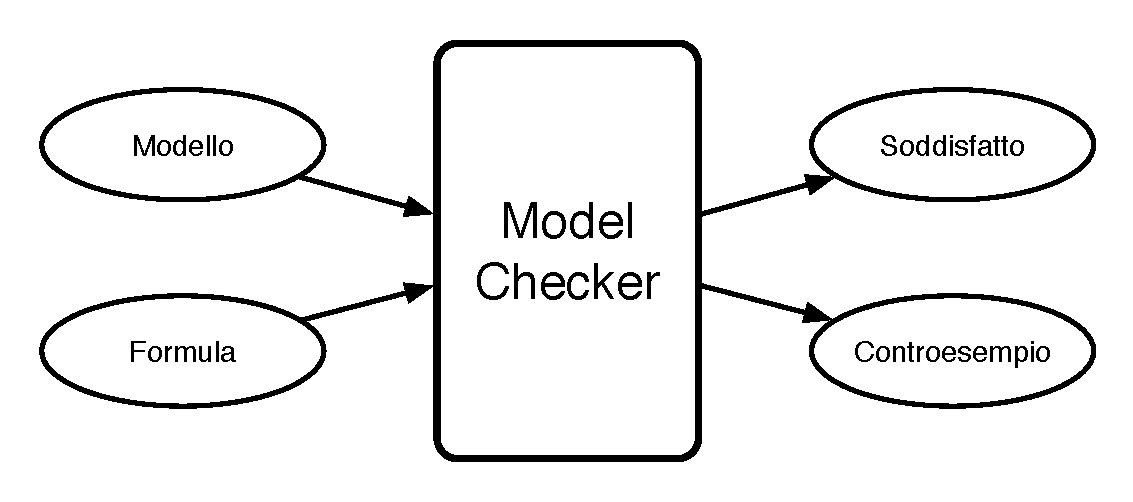
\includegraphics[width=.8\textwidth]{Images/mc.eps}
	\end{center}
\caption{Schema del funzionamento di un model checker}
\label{fig:modelchecker}
\end{figure}

In un contesto reale è spesso impossibile pensare di ottenere un sistema complesso totalmente privo di errori o imperfezioni, si rilassano quindi le richieste introducendo dei gradi di tolleranza degli errori. Un caso concreto può essere il gestore di una compagnia telefonica che permette di effettuare un'alta percentuale di chiamate senza problemi di interferenze o interruzioni, ad esempio il $98\%$. Oltre al modello e alla formula viene quindi introdotto nel model checker il parametro dell'\emph{accuratezza} che rende una formula verificata se il grado di fallimento rientra nella tolleranza espressa. Un model checker a cui si aggiunge un parametro di accuratezza espresso in probabilità viene chiamato \emph{probabilistic model checker} (figura \ref{fig:probabilisticmodelchecker}).
\begin{figure}[htb]
	\begin{center}
		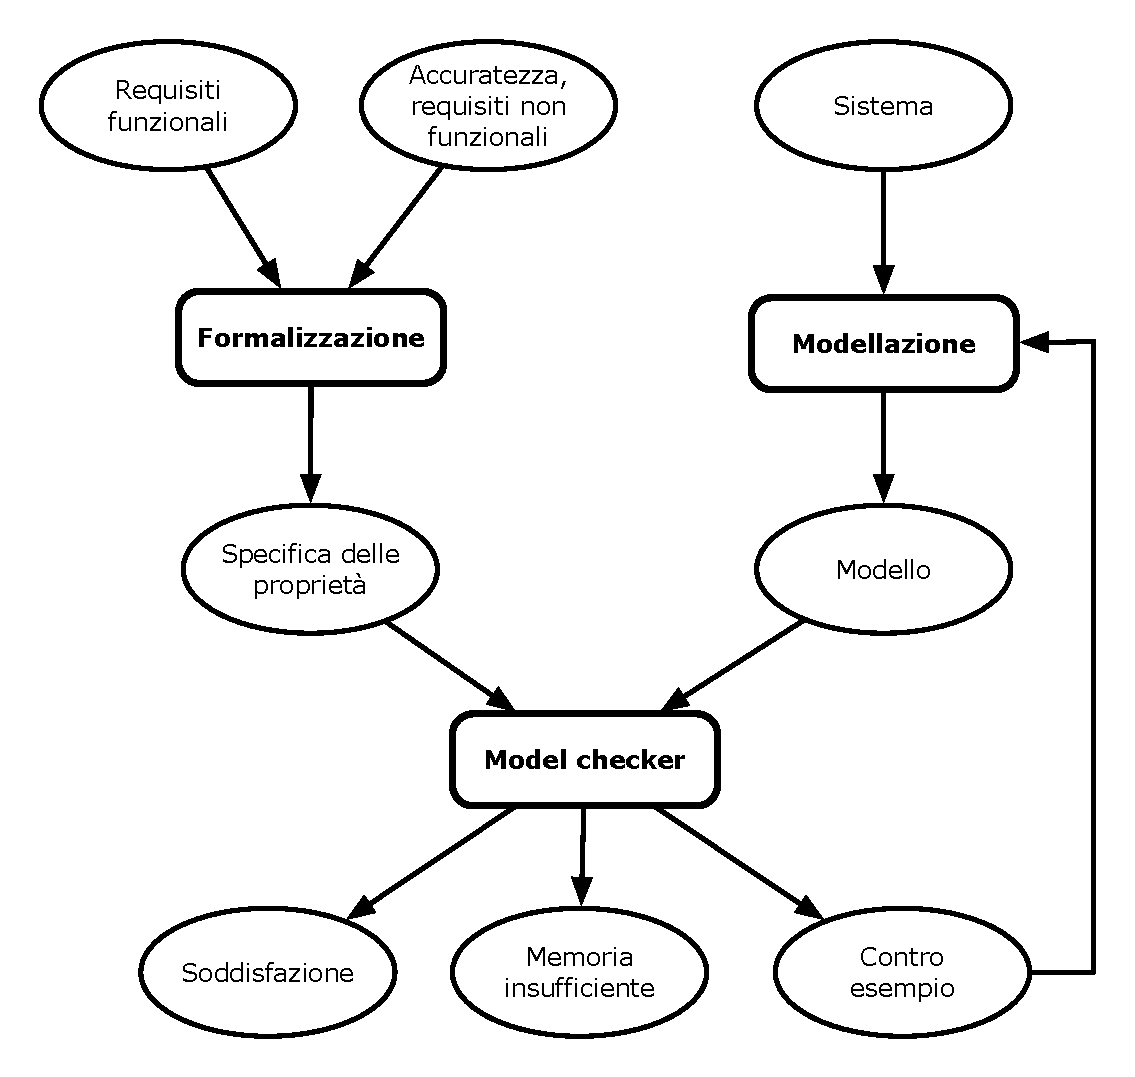
\includegraphics[width=\textwidth]{Images/pmc.eps}
	\end{center}
\caption{Schema del funzionamento di un model checker probabilistico}
\label{fig:probabilisticmodelchecker}
\end{figure}

Dalla formalizzazione dei requisiti si può ottenere un insieme di proprietà che dovranno essere soddisfatte. Più precisamente, dai requisiti \emph{funzionali} possiamo ottenere le formule di proprietà da soddisfare, mentre quelli \emph{non funzionali} forniscono l'accuratezza da utilizzare. Dopo aver fornito al model checker il modello del sistema, la proprietà da verificare e l'accuratezza, questo può produrre tre tipi di risposte:
\begin{itemize}
	\item la proprietà viene soddisfatta dal modello nei limiti richiesti,
	\item la memoria non è sufficiente per portare a termine la verifica oppure
	\item la proprietà non viene soddisfatta dal modello, fornendo un controesempio.
\end{itemize}
Se non si riceve esito positivo si può intervenire a seconda di che tipo di problema è stato riscontrato. Nel secondo caso si verifica il fenomeno conosciuto come \emph{esplosione degli stati} che ha origine quando si vuole modellare sistemi molto complessi, come i già citati software multithread. La conseguenza è una richiesta di memoria e tempo di calcolo proibitivi. Per far fronte a questo problema si ricorre spesso alla scomposizione del sistema in sotto sistemi e ad astrazioni di modelli troppo complessi. Ovviamente se invece non viene soddisfatta la formula è necessario intervenire sul modello stesso cercando di correggere i comportamenti erronei evidenziati.

Il model checking viene utilizzato in modo diverso se ci troviamo prima o dopo la fase di sviluppo: nel primo caso è necessario costruire il modello astratto del sistema, nel secondo, invece, è possibile utilizzare degli strumenti (i.e. \emph{java path finder}) per effettuare le verifiche direttamente sul codice. 

\section{Probabilit\`a elementari}
Introduciamo le misure principali utilizzate dei model checker probabilistici, assumendo di utilizzare come strutture dei modelli le \ac{dtmc} e le \ac{mdp}. Esistono due tipi di misure di probabilità elementari delle \ac{dtmc}:
\begin{itemize}
	\item probabilità \emph{transiente} e
	\item probabilità \emph{a regime}, o \emph{steady state}.
\end{itemize}

\begin{mtdef}[Probabilità transiente $\pi_j(n)$]
La probabilità \emph{transiente} $\pi_j(n) = \mathbb{P}\{X_n = j\}$ è la probabilità che la \ac{dtmc} sia nello stato $j$ al passo $n$
\end{mtdef}

Possiamo quindi associare alla \ac{dtmc} $\mathcal{D}$ un vettore che al passo $n$ descriva la probabilità di trovarsi in ogni stato $s \in S$ $$\underline\pi(n) \triangleq (\pi_1(n), \dots, \pi_{|S|}(n)).$$
Si indica con $\underline\pi(0)$ la distribuzione di probabilità iniziale mentre con $\underline\pi(n)$ la distribuzione di probabilità al passo $n$.
Considerando che moltiplicare il vettore di distribuzione di probabilità per la matrice $\mathbb{P}$ rappresenta un avanzamento del sistema che aggiorna la distribuzione al passo successivo, allora vale la seguente \emph{relazione di ricorrenza}
$$ \underline\pi(n) = \underline\pi(n-1) \cdot \mathbb{P} $$
da cui si ricava immediatamente la seguente forma dipendente solo dalla  distribuzione iniziale e dalla matrice di transizione
$$ \underline\pi(n) = \underline\pi(0) \cdot \mathbb{P}^n$$

\begin{mtdef}[Probabilità steady state $\pi_j$]
La probabilità \emph{steady state} $$\pi_j = \lim_{n\rightarrow\infty} \mathbb{P}\{X_n = j\}$$ è la probabilità che la \ac{dtmc} sia a regime nello stato $j$.
\end{mtdef}

L'esistenza di questo limite è garantita solo sotto determinate condizioni di \emph{ergodicità} della catena. Supponendo che il limite sia indipendente dalla distribuzione iniziale, per calcolare questa distribuzione è sufficiente risolvere il seguente sistema di equazioni lineari
$$
\left\{
\begin{array}{l}
\underline\pi \cdot \mathbb{P} = \underline\pi \\
\sum^{|S|}_{i=1} \pi_i = 1 \\
\end{array}
\right.
$$
dove $0 \leq \pi_i \leq 1$ e $1 \leq i \leq |S|$.

Una volta scelto uno scheduler che risolva le scelte nondeterministiche della \ac{mdp} trasformandola in una \ac{dtmc} sarà possibile applicare la valutazione delle probabilità sopra descritte. Il risultato però sarà valido solo in presenza di quello specifico scheduler che potrebbe avere un peso poco rilevante nell'analisi della \ac{mdp}. Quello che si fa quindi è calcolare il range di probabilità in cui si muove la misura interessata \emph{per ogni} possibile scheduler in modo da poter fare inferenza su \emph{lower} e \emph{upper bounds}.

\section{Probabilistic Computation Tree Logic}
Al fine di poter effettuare model checking su strutture come \ac{dtmc} e \ac{mdp} utilizziamo \ac{pctl}, un'estensione probabilistica della logica temporale \ac{ctl}. Il linguaggio \ac{pctl} è uno strumento che permette di esprimere specifiche di interesse sulla struttura che stiamo condiderando. Può essere quindi utilizzato sia sulle \ac{dtmc} che sulle \ac{mdp} adattando la struttura alla potenza espressiva del modello. In generale le formule che esprimono specifiche in modo formale hanno un ruolo fondamentale all'interno del model checking in quanto permettono di rendere automatico il procedimento di verifica.

In seguito riportiamo la sintassi e la semantica di \ac{pctl} definita per le \ac{mdp}, più generale rispetto a quella per le \ac{dtmc} ed effettivamente impiegata all'interno di questo lavoro.

\begin{mtdef}[Sintassi \ac{pctl}]
	La sintassi \ac{pctl} viene definita come segue:
$$
\begin{array}{rcl}
	\phi &::=& true \Sep \mathit{a} \Sep \phi_1 \wedge \phi_2 \Sep \neg\phi \Sep \mathcal{P}_{\bowtie p}[\psi] \\
	\psi &::=& \mathcal{X}\phi \Sep \phi_1 \mathcal{U}^{\leq k} \phi_2 \Sep \phi_1 \mathcal{U} \phi_2 \\
\end{array}
$$
dove $\mathit{a}$ è una proposizione atomica, $\bowtie \in \{\leq,<,\geq,>\}$, $p \in[0,1]$ e $k \in \mathbb{N}$.
\end{mtdef}
Dalla sintassi distinguiamo due tipi di formula: le formule di stato $\phi$ e le formule di cammino $\psi$. Per definire formalmente la semantica è necessario specificare come gli elementi dell'insieme $AP$ delle proposizioni atomiche sono gestiti in una \ac{mdp}.
\begin{mtdef}[\ac{mdp} etichettata]
	Una \ac{mdp} etichettata è una tupla $(\mathcal{M},L)$ dove:
	\begin{itemize}
		\item $\mathcal{M}$ è una \ac{mdp};
		\item $L:S\rightarrow 2^{AP}$ è una funzione di etichettatura.
	\end{itemize}
\end{mtdef}
Estendiamo quindi la struttura delle \ac{mdp} con una funzione $L$ che associa ad ogni stato un certo insieme di proposizioni atomiche. A questo punto abbiamo tutti gli strumenti per definire la semantica di \ac{pctl} secondo una relazione di soddisfacibilità.
\begin{mtdef}[Relazione di soddisfacibilità]
	Sia $\mathcal{M} = (S,\overline{s},Act,Steps,L)$ una \ac{mdp} etichettata. Per ogni stato $s \in S$, la relazione di soddisfacibilità di stato $\models$ è definita per induzione come segue:
$$
	\begin{array}{rllcl}
		\mathcal{M},s &\models& \phi &\Leftrightarrow& \mathcal{M},s \models_{st} \phi \\
		\mathcal{M},s &\models_{st}& true && \forall s \in S, \\
		\mathcal{M},s &\models_{st}& \mathit{a} &\Leftrightarrow& \mathit{a} \in L(s), \\
		\mathcal{M},s &\models_{st}& \neg\phi &\Leftrightarrow& s \not\models_{st} \phi, \\
		\mathcal{M},s &\models_{st}& \phi_1 \wedge \phi_2 &\Leftrightarrow& s\models_{st}\phi_1 \ e\ s\models_{st}\phi_2, \\
		\mathcal{M},s &\models_{st}& \mathbb{P}\{ \mathcal{P}_{\bowtie p}[\psi]\} &\Leftrightarrow& p_s^\Sigma(\psi)\bowtie p,\ \forall\ \Sigma \in Scheduler_\mathcal{M}, \\
	\end{array}
$$
dove per ogni scheduler $\Sigma \in Scheduler_\mathcal{M}$:
$$
p_s^\Sigma \triangleq Prob_s^\Sigma(\{\pi \in Path_s^\Sigma \sep \pi \models_{pt} \psi\})
$$
e per ogni cammino $\pi \in Path$:
$$
\begin{array}{rclcl}
	\mathcal{M},\pi & \models_{pt} & \mathcal{X}\phi & \Leftrightarrow & \mathcal{M},\pi(1) \models_{pt} \phi, \\
	\mathcal{M},\pi & \models_{pt} & \phi_1 \mathcal{U}^{\leq k} \phi_2 & \Leftrightarrow & \exists i \leq k\ .\ (\mathcal{M},\pi(i) \models_{pt} \phi_2\ e\ \mathcal{M},\pi(j) \models_{pt} \phi_1 \forall j < i), \\
	\mathcal{M},\pi & \models_{pt} & \phi_1 \mathcal{U} \phi_2 & \Leftrightarrow & \exists k \geq 0\ .\ \mathcal{M},\pi \models_{pt} \phi_1 \mathcal{U}^{\leq k} \phi_2. \\
\end{array}
$$
\end{mtdef}

Per specificare una formula \ac{pctl} si utilizza sempre una formula di stato che al suo interno potrà utilizzare formule di cammino. Intuitivamente gli operatori logici possono essere utilizzati per indagare sulle proposizioni atomiche contenute in un determinato stato, mentre l'operatore $\mathcal{P}_{\bowtie p}[\psi]$ viene soddisfatto dagli stati che soddisfano la formula di cammino $\psi$ con una probabilità nell'intervallo specificato da $\bowtie p$. Questo operatore si comporta sempre nel modo appena descritto se i cammini non incontrano scelte nondeterministiche (nelle \ac{dtmc} è sempre vero) ma come deve comportarsi in caso contrario? Dato che non si può assumere niente sulle suddette scelte e sfruttando il fatto che l'applicazione di uno scheduler ad una \ac{mdp} produce una \ac{dtmc}, l'operatore è considerato soddisfatto se la condizione è valida \emph{per qualsiasi scheduler}.

Per quanto riguarda le formule di cammino, l'operatore \emph{next} $\mathcal{X}\phi$ richiede che $\phi$ venga soddisfatta dallo stato successivo, l'operatore \emph{bounded until} $\phi_1 \mathcal{U}^{\leq k} \phi_2$ richiede che $\phi_2$ venga soddisfatto entro $k$ passi e che $\phi_1$ resti sempre soddisfatto fino a quel punto, mentre l'operatore \emph{unbonded until} $\phi_1 \mathcal{U} \phi_2$ richiede che prima o poi $\phi_2$ venga soddisfatto e che $\phi_1$ sia sempre soddisfatto fino a quel punto.

Possiamo rielaborare i construtti principali definiti finora per estendere il linguaggio con degli operatori derivati (tabella \ref{tab:sintassi:derivati}). Mentre gli operatori logici $false$, $\vee$ e $\rightarrow$ possono essere derivati facilmente, vi sono alcuni operatori meno banali. Gli operatori $\Diamond$ e $\Box$ sono molto comuni nelle logiche temporali e servono a specificare rispettivamente proprietà che hanno speranza di avverarsi in futuro e proprietà che sicuramente non si verificheranno mai. Delle applicazioni interessanti di questi due concetti sono le proprietà di \emph{liveness} e di \emph{safety}. Una proprietà di \emph{liveness} esprime la possibilità che prima o poi accada qualcosa di positivo mentre la duale \emph{safety} indica che qualcosa di negativo non potrà mai accadere. I due operatori possono essere usati per descrivere queste due tipologie proprietà ma sono più generali. 
Le varianti \emph{bounded} $\Diamond^{\leq k}$ e $\Box^{\leq k}$ stabiliscono, tramite il numero di passi $k \in \mathbb{N}$, il tempo entro il quale la proprietà $\phi$ deve rimanere soddisfatta a partire dall'istante iniziale. La proprietà di cammino $\Diamond^{\leq k}\phi$ sarà quindi soddisfatta se entro $k$ passi $\phi$ si verificherà almeno una volta, mentre la proprietà di cammino $\Box^{\leq k}$ sarà soddisfatta se $\phi$ rimarrà sempre soddisfatta per tutti e $k$ i passi. 
Per definire gli operatori $\Box$ e $\Box^{\leq k}$ viene introdotta la notazione $\overline\bowtie$ che rappresenta l'inversione degli operatori secondo le seguenti equivalenze: $\overline\leq \equiv \geq$, $\overline < \equiv >$, $\overline\geq \equiv \leq$ e $\overline > \equiv <$.
Un ultimo operatore interessante è il quantificatore esistenziale $\exists$ che \emph{ricerca l'esistenza di uno scheduler} che soddisfa una certa formula, contrariamente all'approccio generale basato sulla soddisfacibilità di tutti i possibili scheduler.
\begin{table}[htbp!]
$$
\begin{array}{rcl}
	false & \equiv & \neg true \\
	\phi_1 \vee \phi_2 & \equiv & \neg(\neg\phi_1 \wedge \neg\phi_2) \\
	\phi_1 \rightarrow \phi_2 & \equiv & \neg\phi_1 \vee \phi_2 \\
	\mathcal{P}_{\bowtie p}[\Diamond \phi] & \equiv & \mathcal{P}_{\bowtie p}[true \mathcal{U} \phi] \\
	\mathcal{P}_{\bowtie p}[\Diamond^{\leq k} \phi] & \equiv & \mathcal{P}_{\bowtie p}[true \mathcal{U}^{\leq k} \phi] \\
	\mathcal{P}_{\bowtie p}[\Box \phi] & \equiv & \mathcal{P}_{\overline\bowtie 1-p}[\Diamond \neg \phi] \\
	\mathcal{P}_{\bowtie p}[\Box^{\leq k} \phi] & \equiv & \mathcal{P}_{\overline\bowtie 1-p}[\Diamond^{\leq k} \neg \phi] \\
	\exists\Diamond\phi & \equiv & \neg \mathcal{P}_{\leq 0}[\Diamond\phi] \\
\end{array}
$$
\caption{Operatori derivati di \acs{pctl}}
\label{tab:sintassi:derivati}
\end{table}

\section{PRISM model checker}
Il model checker probabilistico che utilizzeremo è \prism{} \cite{KNP11}. Si tratta di un tool con il quale è possibile fare modellazione e analisi di sistemi che presentano aspetti probabilistici. I principali modelli probabilistici supportati sono le \ac{dtmc}, le \ac{mdp}, le \ac{ctmc} ed i \ac{pta}, mentre i linguaggi utilizzabili per descrivere le formule sono \ac{pctl}, \ac{csl} e \ac{ltl}. In questa sezione descriveremo l'utilizzo di \prism{} concentrandoci sugli strumenti di interesse diretto per questo lavoro come le \ac{mdp} e il linguaggio \ac{pctl} precedentemente descritti.

\prism{} utilizza un suo specifico linguaggio con il quale è possibile definire tutti i modelli sopra citati. Si tratta infatti di un linguaggio basato sugli stati e su formalismi tipici dei sistemi reattivi. I componenti fondamentali rappresentati dal linguaggio sono i \emph{moduli} e le \emph{variabili}, un \emph{modello} viene rappresentato come un insieme di moduli che possono interagire tra loro. Ogni modulo può inoltre contenere delle variabili locali e il valore di queste variabili ad un certo istante rappresentano il suo stato. Allo stesso modo lo stato del modello globale è definito come lo stato locale di tutti i moduli che lo compongono.

Il comportamento di un modulo viene definito dall'insieme di \emph{comandi} che contiene. Un comando ha la seguente forma:
\begin{verbatim}
	[] guardia -> prob_1 : update_1 + ... + prob_n : update_n ;
\end{verbatim}
La \emph{guardia} è un predicato che può considerare qualsiasi variabile del modello e se risulta soddisfatta il modello può avanzare eseguendo una delle transizioni \emph{update} con le rispettive probabilità (o evenutalmente rate). L'intero modulo viene definito specificandone il nome e il contenuto
\begin{verbatim}
	module name ... endmodule
\end{verbatim}
All'interno del modulo possono essere presenti sia comandi che variabili. Al fine di avere uno \emph{spazio finito di stati} \prism{} permette di gestire solo variabili booleane e variabili intere in un range finito. Di seguito mostriamo la dichiarazione di una variabile $x$ che può assumere i valori interi compresi tra $0$ e $10$ compresi inizializzata a 5 e una variabile booleana $b$ inizializzata a $true$:
\begin{verbatim}
	x : [0..10] init 5;
	b : bool init true;
\end{verbatim}
Le guardie sono classiche espressioni booleane che possono fare riferimento a variabili di qualsiasi modulo in quanto viene richiesta solamente la lettura dei valori. Gli update, invece, sono sequenze di assegnamenti intervallate dal separatore $\&$. La sequenza di update vuota viene indicata con $true$. Un assegnamento di un valore a una variabile può avvenire solo su una variabile locale al modulo a cui appartiene il comando, inoltre il nome della variabile aggiornata deve terminare col simbolo $'$ ad indicarne il nuovo stato. All'interno del listato \ref{code:prism:example1} mostriamo l'utilizzo degli strumenti appena descritti. L'esempio rappresenta due processi in mutua esclusione.
\begin{lstlisting}[language=prism,style=eclipse,caption={Esempio di definizione dei moduli in \prism{}},label=code:prism:example1]
module M1

x : [0..2] init 0;

    [] x=0 -> 0.8:(x'=0) + 0.2:(x'=1);
    [] x=1 & y!=2 -> (x'=2);
    [] x=2 -> 0.5:(x'=2) + 0.5:(x'=0);

endmodule 

module M2

y : [0..2] init 0;

    [] y=0 -> 0.8:(y'=0) + 0.2:(y'=1);
    [] y=1 & x!=2 -> (y'=2);
    [] y=2 -> 0.5:(y'=2) + 0.5:(y'=0);

endmodule
\end{lstlisting}
In questo caso i due moduli sono simmetrici, ed entrambi presentano esclusivamente scelte probabilistiche. Possiamo se necessario inserire anche delle scelte non deterministiche sulle quali è quindi impossibile fare osservazioni di tipo quantitativo. Modificando il modulo $M1$ come mostrato nel listato \ref{code:prism:example2} inseriamo una scelta nondeterministica, infatti le due nuove guardie insierite saranno sempre abilitate insieme.
\begin{lstlisting}[language=prism,style=eclipse,caption={Scelta nondeterministica in \prism{}},label=code:prism:example2]
module M1

x : [0..2] init 0;

	// scelta nondeterministica
    [] x=0 -> (x'=0);
	[] x=0 -> (x'=1);
	
    [] x=1 & y!=2 -> (x'=2);
    [] x=2 -> 0.5:(x'=2) + 0.5:(x'=0);
	
endmodule
\end{lstlisting}
In generale il nondeterminismo può verificarsi anche se due guardie vengono soddisfatte assieme anche solo parzialmente. La stessa struttura può quindi presentare scelte deterministiche a seconda dello stato corrente.

In \prism{} è anche possibile definire delle costanti globali sui domini di interi, reali e booleani:
\begin{verbatim}
	const int z = 12;
	const double pi = 3.141592;
	const bool flag = true;
\end{verbatim}
Queste costanti possono essere utilizzate, al fine di parametrizzare il modello, all'interno delle espressioni che possono coinvolgere i seguenti operatori:
\begin{itemize}
	\item $-$ meno unario, $*$ moltiplicazione, $\slash$ divisione, $+$ somma e $-$ sottrazione,
	\item le relazioni d'ordine $<$, $\leq$, $>$, $\geq$, e di equivalenza $=$ e $!=$
	\item gli operatori booleani di $!$ negazione, $\&$ congiunzione, $|$ disgiunzione, $<=>$ se e solo se e $=>$ implicazione logica.
\end{itemize}
Sono presenti inoltre le funzioni:
\begin{itemize}
	\item $min$ minimo e $max$ massimo,
	\item $floor$ di arrotondamento all'intero minore più vicino,
	\item $ceil$ di arrotondamento all'intero maggiore più vicino,
	\item $pow$ per l'elevamento a potenza,
	\item $mod$ modulo,
	\item $log$ logaritmo.
\end{itemize}
Le espressioni possono essere utilizzate non solo nelle condizioni delle guardie, nelle inizializzazioni e negli aggiornamenti, ma anche per calcolare le proprietà di una transizione.

Come primo parametro di un comando può essere inserita la label di un'azione per far sincronizzare i moduli. Un azione viene quindi specificata inserendone il nome (ad esempio \emph{step}) all'interno delle parentesi quadre, nel seguente modo
\begin{verbatim}
	[step] x=0 -> 0.8:(x'=0) + 0.2:(x'=1);
\end{verbatim}

Il modello finale viene ricavato di default dalla \emph{composizione parallela} di tutti i moduli che lo compongono, se si vuole invece descrivere una composizione diversa, è possibile usare il costrutto
\begin{verbatim}
	system ... endsystem
\end{verbatim}
Al suo interno possono essere usati i seguenti operatori \ac{csp}:
\begin{itemize}
	\item $M1\ ||\ M2$: i moduli si sincronizzano solo su azioni che appaiono in entrambi (composizione parallela di default),
	\item $M1\ |||\ M2$: interleaving completo, senza sincronizzazione,
	\item $M1\ |[a,b,...]|\ M2$: la sincronizzazione avviene solo sulle azioni specificate nell'operatore,
	\item $M \slash \{a,b,...\}$ le azioni specificate vengono nascoste all'esterno,
	\item $M \{a<-b,c<-d,...\}$ le azioni vengono rinominate all'esterno.
\end{itemize}
Alcuni esempi di espressioni di sistema sono mostrati di seguito:
\begin{verbatim}
	system (station1 ||| station2 ||| station3) |[serve]| server endsystem
	system ((P1 |[a]| P2) / {a}) || Q endsystem
	system ((P1 |[a]| P2) {a<-b}) |[b]| Q endsystem
\end{verbatim}

%!TEX root = ../main.tex

\myChapter{PRISM}
\cleardoublepage\myPart{LAPSA: un linguaggio per agenti adattivi}
%!TEX root = ../main.tex

% TODO box delle sintassi
% TODO box della semantica finale
% TODO parentesi nelle condizioni
% TODO ricontrollare le sintassi che siano uguali
% TODO traduzione codice: copiare direttamente da xtext?
% TODO acronimi: invertire la prima comparsa
% TODO citazione a inizio capitolo: LAPSA -> volpe in léttone

\myChapter{LAPSA}

Per definire ed implementare un modello di un sistema adattivo possono essere utilizzati molti strumenti già esistenti. L'approccio che vogliamo impiegare coinvolge l'utilizzo di un model checker come supporto alle scelte che possiamo semplicemente scegliere a seconda delle specifiche e delle esigenze dello scenario.

In questo capitolo viene introdotta la definizione del linguaggio \ac{lapsa}, un linguaggio specifico per agenti adattivi. L'obiettivo che si vuole raggiungere con questo linguaggio è definire un'interfaccia che permetta di modellare sistemi adattivi in modo più efficiente ed efficace possibile. Si parla di interfaccia in quanto, attraverso la definizione di sintassi e semantica, si dichiara \emph{cosa} possono fare i costrutti linguistici di \ac{lapsa} (front-end) senza entrare in merito del \emph{come} questo verrà implementato (back-end).

Il back-end è stato implementato in \java{} tramite \xtext{} \cite{xtext}, un meta-tool specifico per la creazione di plugin \eclipse{} di linguaggi personalizzati. Definendo la grammatica del proprio linguaggio è possibile implementarne velocemente la traduzione del codice ed i servizi di utilità più diffusi come l'autocompletamento e la colorazione delle parole chiave. Oltre al compilatore è presente anche il model checker \prism{} in grado di eseguire i controlli di formule \ac{pctl} su \ac{mdp} definite secondo il suo specifico linguaggio.

L'approccio utilizzato separa il linguaggio dal livello implementativo permettendo di cambiare gli strumenti sottostanti senza che l'utilizzatore debba venirne a conoscenza, a patto che i nuovi strumenti rispettino la semantica dei costrutti linguistici.

\section{Sintassi}
Per descrivere la sintassi \ac{lapsa} sarà utilizzato il formalismo \emph{EBNF} indicando con le parole in corsivo i simboli non terminali e con quelle in neretto e quelle in stampatello i non terminali. Le parole in neretto sono \emph{keyword} del linguaggio mentre quelle in stampatello descrivono dei valori arbitrari su insiemi come nomi di variabili o costanti numeriche. Procederemo con la descrizione informale di cosa viene identificato con i costrutti sintattici del linguaggio introducendoli gradualmente.

Il non terminale \emph{program} è il simbolo iniziale della grammatica e nella sua struttura racchiude la dichiarazione dell'insieme di azioni considerato, il modulo che descrive il comportamento del soggetto, i moduli che possono essere usati per descrivere l'ambiente e i dati necessari alla discretizzazione delle variabili (tabella \ref{tab:lapsaProgram}).

\begin{table}[htbp!] % sintassi programma LAPSA
$$
\begin{array}{rcl}
	\mathit{program} &::=& \mathbf{actions} \Space \{ \mathit{actions} \} \\
		&& \mathbf{subject} \Space \mathit{module} \\
		&& \mathit{modules} \\
		&& \mathit{environment} \\
		&& \mathbf{ranges} \Space \{ \mathit{ranges} \} \\
\end{array}
$$
\caption{Sintassi \ac{lapsa} di \emph{program}}
\label{tab:lapsaProgram}
\end{table}

Il non terminale \emph{actions} è una semplice lista dove vengono dichiarate i nomi delle azioni che possono essere effettuate (tabella \ref{tab:lapsaActions}). Ovviamente le azioni utilizzate in seguito nelle transizioni dei moduli e nelle sincronizzazioni dovranno essere state dichiarate in questa sezione per considerare il programma \emph{corretto}.

\begin{table}[htbp!] % sintassi azioni LAPS
$$
\begin{array}{rcl}
	\mathit{actions} &::=& \x{action}\textrm{-}\x{id} \Sep \mathit{actions} \Space \mathit{actions} \\
\end{array}
$$
\caption{Sintassi \ac{lapsa} di \emph{actions}}
\label{tab:lapsaActions}
\end{table}

La definizione di un comportamento viene espressa tramite il non terminale \emph{module} che permette di descrivere i suoi dati, le sue transizioni e i suoi obiettivi (tabella \ref{tab:lapsaModule}). I dati sono rappresentati dalla lista \emph{variables} e ogni dato è rappresentato dal tipo di dato, il nome associato e l'espressione che gli attribuisce un valore iniziale. Con il non terminale \emph{rules}, invece, viene descritta una lista di transizioni. Le transizioni vengono definite come la tripla \emph{condizione}, \emph{azione}, \emph{distribuzione}: se la condizione è vera allora può essere effettuata l'azione e l'aggiornamento dello stato secondo la distribuzione di probabilità. Gli obiettivi vengono descritti nella lista \emph{targets} dove il primo criterio ha importanza massima e decrementa fino all'ultimo che sarà il meno importante.

\begin{table}[htbp!] % sintassi modulo LAPSA
$$
\begin{array}{rcl}
	\mathit{module} &::=& \mathbf{module} \Space \x{module}\textrm{-}\x{id} \Space \{ \mathit{variables} \Space \mathit{rules} \Space \mathit{targets} \}
		\\[.3cm]
	\mathit{variables} &::=& \x{type} \Space \x{variable}\textrm{-}\x{id} = \mathit{expression}; \Sep \mathit{variables} \Space \mathit{variables}
		\\[.3cm]
	\mathit{rules} &::=& \mathit{condition} [ \x{action}\textrm{-}\x{id}] \Rightarrow \mathit{distribution}; \Sep \mathit{rules} \Space \mathit{rules}
		\\[.3cm]
	\mathit{targets} &::=& \mathbf{target} \Space \mathbf{never} \Space \mathit{condition} \Sep \mathit{targets} \Space \mathit{targets} \\
\end{array}
$$
\caption{Sintassi \ac{lapsa} di \emph{module} e delle sezioni che lo compongono}
\label{tab:lapsaModule}
\end{table}

Le distribuzioni di probabilità (tabella \ref{tab:lapsaDistribution}) sono definite come un insieme di possibili aggiornamenti dello stato associati ad un certo valore di probabilità. Questo valore viene espresso nel costrutto sintattico dall'espressione all'interno delle parentesi angolate e viene normalizzato con gli altri nel caso in cui la somma non sia $1$. Questi valori possono anche dipendere dalle variabili di stato e quindi variare con l'avanzamento del modello.

\begin{table}[htbp!] % sintassi delle distribuzioni in LAPSA
$$
\begin{array}{rcl}
	\mathit{distribution} &::=& <\mathit{expression}> \mathit{update} \Sep \mathit{distribution} \Space \# \Space \mathit{distribution} \\
\end{array}
$$
\caption{Sintassi \ac{lapsa} di \emph{distribution}}
\label{tab:lapsaDistribution}
\end{table}

Ogni caso di una distribuzione porta a una lista di aggiornamenti che possono essere descritti con i costrutti sintattici definiti in tabella \ref{tab:lapsaUpdate}. Si può modificare il valore di una variabile tramite assegnamento o specificare che nessun cambiamento verrà eseguito tramite l'operazione nulla \texttt{noaction}. Per mezzo degli operatori \texttt{env.add} e \texttt{env.remove} è possibile agire sull'ambiente aggiungendo e rimuovendo elementi rispettivamente.

\begin{table}[htbp!] % sintassi degli aggiornamenti in LAPSA
$$
\begin{array}{rcl}
	\mathit{update} &::=& \x{variable}\textrm{-}\x{id} = \mathit{expression} \Sep \mathbf{noaction} \\
		& \Sep & \mathit{update} \Space , \Space \mathit{update} \\
\end{array}
$$
\caption{Sintassi \ac{lapsa} di \emph{update}}
\label{tab:lapsaUpdate}
\end{table}

Il non terminale \emph{modules} descritto, assieme ad \emph{environment}, in tabella \ref{tab:lapsaModules} viene utilizzato per definire un insieme di moduli che poi potranno essere istanziati nell'ambiente con dei riferimenti al loro nome. Questo accade all'interno del non terminale \emph{environment} dove viene descritto l'ambiente come una lista di riferimenti a moduli intervallati dagli insiemi di azioni su cui possono sincronizzarsi, un operatore che riprende sintatticamente e semanticamente dal parallelo di Hoare in \ac{csp} \cite{Hoare:1978:CSP}.

\begin{table}[htbp!] % sintassi della definizione dei moduli e dell'ambiente in LAPSA
$$
\begin{array}{rcl}
	\mathit{modules} &::=& \mathit{module} \Sep \mathit{modules} \Space \mathit{modules}
		\\[.3cm]
	\mathit{environment} &::=& \x{module}\textrm{-}\x{id} \Sep \mathit{environment} \Par{\{\mathit{actions}\}} \mathit{environment}
		\\
\end{array}
$$
\caption{Sintassi \ac{lapsa} di \emph{modules} e di \emph{environment}}
\label{tab:lapsaModules}
\end{table}

Le condizioni hanno un ruolo importante in quanto parte fondamentale dell'abilitazione delle transizioni. La sintassi di una condizione è illustrata in tabella \ref{tab:lapsaCondition} e mette a disposizione, oltre ai costrutti sintattici più classici come gli operatori booleani e il confronto tra espressioni, anche il quantificatore esistenziale. Questo operatore viene considerato soddisfatto se esiste un modulo del tipo specificato che soddisfa la condizione espressa. La condizione del quantificatore esistenziale può fare riferimento al nome temporaneo associato al tipo di modulo interessato in modo da poter indagare sulle sue variabili di stato.

\begin{table}[htbp!] % sintassi delle condizioni in LAPSA
$$
\begin{array}{rcl}
	\mathit{condition} &::=& \mathbf{exists} \Space \x{variable}\textrm{-}\x{id}:\x{module}\textrm{-}\x{id} \Space \mathbf{such}\Space\mathbf{that} \Space \mathit{condition} \\
		& \Sep & \mathit{expression} \bowtie \mathit{expression} \Sep \mathbf{true} \\
		& \Sep & \mathit{condition} \Space \mathbf{or} \Space \mathit{condition} \Sep \mathbf{not} \Space \mathit{condition}
		\\
\end{array}
$$
\caption{Sintassi \ac{lapsa} di \emph{condition}}
\label{tab:lapsaCondition}
\end{table}

Il simbolo $\bowtie$ rappresenta l'operatore di confronto e può essere quindi definito come $\bowtie = \{<,\leq,>,\geq, =, \neq\}$. Le espressioni (tabella \ref{tab:lapsaExpression}) sono fondamentalmente variabili e costanti numeriche combinate tra loro tramite i classici operatori binari e gli operatori di confronto seguono l'interpretazione classica.
Le variabili referenziate devono essere precedute dall'istanza di appartenenza: se fanno riferimento al modulo nel quale vengono richiamate si utilizza la keyword \texttt{this}, altrimenti il riferimento al modulo interessato nel caso in cui si stia esprimendo una condizione interna ad un quantificatore esistenziale.

\begin{table}[htbp!] % sintassi delle espressioni in LAPSA
$$
\begin{array}{rcl}
	\mathit{expression} &::=& \mathit{expression} \Space \mathit{bop} \Space \mathit{expression} \Sep \mathit{reference} \\
	& \Sep & (\mathit{expression}) \Sep \x{constant}
	\\[.3cm]
	\mathit{reference} &::=& (\x{variable}\textrm{-}\x{id} \Sep \mathbf{this})\mathbf{.} \x{variable}\textrm{-}\x{id}
	\\[.3cm]
	\mathit{bop} &::=& + \Sep - \Sep * \Sep \slash
	\\
\end{array}
$$
\caption{Sintassi \ac{lapsa} di \emph{expression}}
\label{tab:lapsaExpression}
\end{table}

Infine il non terminale \emph{ranges} (tabella \ref{tab:lapsaRanges}) permette di descrivere i range di tutte le variabili dei moduli. Questo costrutto è stato inserito in aggiunta alla normale interfaccia di \ac{lapsa} per adattarne l'implementazione del backend a \prism{} che necessita la conoscenza dei possibili valori delle variabili.

In tabella \ref{tab:lapsaSyntax} viene riportata la sintassi completa di \ac{lapsa} i cui costrutti possono essere estesi 

\begin{table}[htbp!] % sintassi dei range in LAPSA
$$
\begin{array}{rcl}
	\mathit{ranges} &::=& \mathit{reference} \Space \mathbf{in} [\x{constant}, \x{constant}] \Sep \mathit{ranges}, \mathit{ranges} \\
\end{array}
$$
\caption{Sintassi \ac{lapsa} di \emph{ranges}}
\label{tab:lapsaRanges}
\end{table}

\begin{table}[htbp!] % sintassi completa LAPSA
$$
	\begin{array}{|rcl|}
	\hline
	\mathit{program} &::=& \mathbf{actions} \Space \{ \mathit{actions} \} \\
		&& \mathbf{subject} \Space \mathit{module} \\
		&& \mathit{modules} \\
		&& \mathit{environment} \\
		&& \mathbf{ranges} \Space \{ \mathit{ranges} \} 
	\\[.3cm]
	\mathit{actions} &::=& \x{action}\textrm{-}\x{id} \Sep \mathit{actions} \Space \mathit{actions} 
	\\[.3cm]
	\mathit{module} &::=& \mathbf{module} \Space \x{module}\textrm{-}\x{id} \Space \{ \mathit{variables} \Space \mathit{rules} \Space \mathit{targets} \}
	\\[.3cm]
	\mathit{variables} &::=& \x{type} \Space \x{variable}\textrm{-}\x{id} = \mathit{expression}; \Sep \mathit{variables} \Space \mathit{variables}
	\\[.3cm]
	\mathit{rules} &::=& \mathit{condition} [ \x{action}\textrm{-}\x{id}] \Rightarrow \mathit{distribution}; \Sep \mathit{rules} \Space \mathit{rules}
	\\[.3cm]
	\mathit{targets} &::=& \mathbf{target} \Space \mathbf{never} \Space \mathit{condition} \Sep \mathit{targets} \Space \mathit{targets} 
	\\[.3cm]
	\mathit{distribution} &::=& <\mathit{expression}> \mathit{update} \Sep \mathit{distribution} \Space \# \Space \mathit{distribution} 
	\\[.3cm]
	\mathit{update} &::=& \x{variable}\textrm{-}\x{id} = \mathit{expression} \Sep \mathbf{noaction} \\
		& \Sep & \mathit{update} \Space , \Space \mathit{update} 
	\\[.3cm]
	\mathit{modules} &::=& \mathit{module} \Sep \mathit{modules} \Space \mathit{modules}
	\\[.3cm]
	\mathit{environment} &::=& \x{module}\textrm{-}\x{id} \Sep \mathit{environment} \Par{\{\mathit{actions}\}} \mathit{environment}
	\\[.3cm]
	\mathit{condition} &::=& \mathbf{exists} \Space \x{variable}\textrm{-}\x{id}:\x{module}\textrm{-}\x{id} \Space \mathbf{such}\Space\mathbf{that} \Space \mathit{condition} \\
		& \Sep & \mathit{expression} \bowtie \mathit{expression} \Sep \mathbf{true} \\
		& \Sep & \mathit{condition} \Space \mathbf{or} \Space \mathit{condition} \Sep \mathbf{not} \Space \mathit{condition}
	\\[.3cm]
	\mathit{expression} &::=& \mathit{expression} \Space \mathit{bop} \Space \mathit{expression} \Sep \mathit{reference} \\
	& \Sep & (\mathit{expression}) \Sep \x{constant}
	\\[.3cm]
	\mathit{reference} &::=& \x{variable}\textrm{-}\x{id}\mathbf{.}\x{variable}\textrm{-}\x{id} \Sep \mathbf{this}\mathbf{.}\x{variable}\textrm{-}\x{id}
	\\[.3cm]
	\mathit{bop} &::=& + \Sep - \Sep * \Sep \slash
	\\[.3cm]
	\mathit{ranges} &::=& \x{module}\textrm{-}\x{id}\mathbf{.}\x{variable}\textrm{-}\x{id} \Space \mathbf{in} [\x{constant}, \x{constant}] \Sep \mathit{ranges}, \mathit{ranges} 
	\\
	\hline
	\end{array}
$$
\caption{Sintassi di \ac{lapsa}}
\label{tab:lapsaSyntax}
\end{table}

\section{Zucchero sintattico}
La sintassi presentata in tabella \ref{tab:lapsaSyntax} è concreta ma contiene solo gli operatori primitivi ed è dunque solo il nucleo del linguaggio che si vuole utilizzare. Al fine di aumentare la semplicità di comprensione e di scrittura del linguaggio \ac{lapsa} intrudiciamo alcuni costrutti di utilità come una rielaborazione di quelli primitivi già presenti.

Con gli operatori logici possiamo ridefinire i seguenti costrutti all'interno del non terminale \emph{condition}, assumendo $\alpha$ come un $\x{variable}\textrm{-}\x{id}$, $\gamma$ come un $\x{module}\textrm{-}\x{id}$ e $\beta,\beta' \in \mathit{condition}$
$$
\begin{array}{l}
	\mathbf{false} \equiv \mathbf{not} \Space \mathbf{true}
	\\[.3cm]
	\beta \Space \mathbf{and} \Space \beta' \equiv \mathbf{not} \Space (\mathbf{not} \Space \beta \Space \mathbf{or} \Space \mathbf{not} \Space \beta')
	\\[.3cm]
	\mathbf{forall} \Space \alpha:\gamma \Space \mathbf{such} \Space \mathbf{that} \Space \beta \equiv \mathbf{not} \Space \mathbf{exists} \Space \alpha:\gamma \Space \mathbf{such} \Space \mathbf{that} \Space \mathbf{not} \Space \beta
	\\
\end{array}
$$

Inseriamo un costrutto di \emph{rule} tale da poter inserire una condizione di abilitazione dei singoli casi delle distribuzioni, assumendo $\alpha$ come un $\x{action}\textrm{-}\x{id}$, $\beta, \beta' \in \emph{condition}$, $\delta \in \mathit{distribution}$ ed $\epsilon \in \mathit{expression}$
$$
\beta [\alpha] \Rightarrow <\epsilon,\beta'> \alpha \Space \# \Space \delta
\equiv
\beta \Space \mathbf{and} \Space \beta' [\alpha]\Rightarrow <\epsilon> \alpha \Space \# \Space \delta,
\beta \Space \mathbf{and} \Space \mathbf{not} \Space \beta' [\alpha]\Rightarrow \delta
$$

Dato che in \ac{lapsa} è presente il non determinismo se più guardie sono abilitate allo stesso passo, introduciamo la possibilità di scrivere più distribuzioni con una sola guardia che vale per tutte le regole. Sia $\alpha$ un $\x{action}\textrm{-}\x{id}$, $\beta \in \mathit{condition}$ e $\delta,\delta' \in \mathit{distribution}$, introduciamo il seguente costrutto del non terminale \emph{rule}
$$
\beta [\alpha] \Rightarrow \delta \Rightarrow \delta';
\equiv
\beta [\alpha] \Rightarrow \delta; \beta [\alpha] \Rightarrow \delta'; 
$$

Possiamo ottenere con facilmente il costrutto che esprime un obiettivo che vogliamo mantenere durante tutta l'esecuzione:
$$
	\mathbf{target}\ \mathbf{always}\ \mathit{condition} \equiv \mathbf{target}\ \mathbf{never}\ \mathbf{not}\ \mathit{condition}
$$

Infine, per quanto riguarda i riferimenti a variabile, è possibile assumere in assenza del prefisso di appartenenza che la variabile appartenga al modulo locale di default:
$$
	\x{variable}\textrm{-}\x{id} \equiv \mathbf{this}.\x{variable}\textrm{-}\x{id}
$$

%------------------------------------------------------------------------------------
% SEMANTICA
%------------------------------------------------------------------------------------
\section{Semantica}
Durante la descrizione della sintassi sono stati presentati informalmente i costrutti di \ac{lapsa}, passiamo adesso a dare una definizione formale della loro semantica. Rappresenteremo il significato di un programma \ac{lapsa} tramite una \ac{mdp} perché permette di esprimere le transizioni tra stati come scelte nondeterministiche di distrubuzioni di probabilità aventi come supporto l'insieme degli stati stessi.

Ad ogni nonterminale \emph{module} sarà associata una \ac{mdp} della forma
$$ M = (\Sigma,Act,\rightarrow_\rho,\sigma_0) $$
Le parti che compongono la \ac{mdp} sono descritte in seguto, tenendo conto che ogni riferimento ai nodi della sintassi viene inteso come appartenente al modulo in questione e, per semplicità, utilizziamo la notazione $eval(e)$ con $e \in \mathit{expression}$ per indicare la valutazione di un'espressione nel modo classico. 
\begin{itemize}
	\item $\Sigma = \{\sigma \sep \sigma : \mathbb{VAR} \rightarrow \mathbb{VAL}\}$ è l'insieme degli \emph{stati} rappresentati da funzioni che mappano variabili in valori, dove $\mathbb{VAR}$ è l'insieme delle $\x{variable}\textrm{-}\x{id}$ definite nel modulo e $\mathbb{VAL} \subset \mathbb{N}_0$ di cardinalità finita
	\item $\sigma_0 \in \Sigma$ è lo \emph{stato iniziale} del modulo ottenuto tramite la valutazione delle espressioni di dichiarazione,
	$$ \sigma_0(v) = eval(e)$$
	dove ``$\x{type} \Space v = e$''$\in \mathit{variables}$
	\item $Act$ é l'insieme delle azioni $\x{action}\textrm{-}\x{id}$
	\item $\rho \subseteq \space \mathit{condition} \space \times Act \times Dist(U)$ è la \emph{struttura statica} della \ac{mdp} definita come
	$$
	\begin{array}{rcl}
		\rho &=& \{(g,a,d)\ |\ ``g[a] \Rightarrow <e_1> \alpha_1 \# \dots \# <e_n> \alpha_n \ '' \in \mathit{rule}, \\
		&& d=[u_{\alpha_{1}}:p_1, \dots, u_{\alpha_{n}}:p_n]\} \\
	\end{array}
	$$
	dove, per $i=1,\dots,n$, valgono $\alpha_i \in \mathit{update}$, $e_i \in \mathit{expression}$ e la normalizzazione delle probabilità
	$$ p_i = \frac{eval(e_i)}{\sum_{j=1}^{n}eval(e_j)}$$
	\item $U = \{u \sep u : \mathit{update} \times \Sigma \rightarrow \Sigma \}$ è l'insieme delle funzioni di aggiornamento di stato definite come
	$$ 
	u_\alpha(\sigma) = \left\{
	\begin{array}{ll}
		\sigma[eval(e)/x]	& \mbox{se } \alpha = ``x = e'' \\
		\sigma				& \mbox{se } \alpha = ``\mathbf{noaction}'' \\
		u_{\alpha_2}(u_{\alpha_1}(\sigma))	& \mbox{se } \alpha = ``\alpha_1 \alpha_2 \ '' \\
	\end{array}
	\right.
	$$
	dove $\alpha, \alpha_1, \alpha_2 \in \mathit{update}$, $\sigma \in \Sigma$, $x \in \mathbb{VAR}$ ed $e \in \mathit{expression}$
	\item $\rightarrow_\rho \subseteq \Sigma \times Act \times Dist(U)$ è la relazione di \emph{avanzamento}: questa relazione descrive come evolve lo stato del modulo col passare del tempo, e viene descritto dalla seguente regola di inferenza
	$$
	\begin{array}{cl}
		\displaystyle{\frac{(g,a,d) \in \rho}{\sigma \xrightarrow{a}_\rho d(\sigma)} \Space \sigma \models g} & \mbox{(Update 1)} \\
	\end{array}
	$$
\end{itemize}

Salendo dal livello dei moduli a quello del sistema globale inteso come la composizione parallela del modulo \emph{subject} con l'ambiente, introduciamo $\Pi \in Dist(S)$ per indicare distribuzioni di sistemi. Un sistema $S$ è un insieme che contiene tutti i moduli riferiti in \emph{environment} (eventualmente anche con più istanze dello stesso modulo) e il modulo principale \emph{subject}. Consideriamo quindi per semplicità la semantica definita su $S$ come nonterminale fittizio
$$ S ::= \x{module}\textrm{-}\x{id} \Sep S_1 \Space |\{\mathit{actions}\}| \Space S_2 $$

Possiamo utilizzare $S$ per descrivere il come \ac{lapsa} gestisce la composizione del modulo principale con quelli dell'ambiente.
$$ \x{subject}\textrm{-}\x{id} \Space |\{\mathit{Act}\}| \Space \mathit{environment} $$

Le regole di inferenza riportate di seguito descrivono la semantica di $S$ in quanto più generale e comprensibile, dalla quale si può facilmente derivare il comportamento specifico. Useremo le notazioni $\sigma_m$ e $\rho_m$ per indicare rispettivamente lo stato e la struttura statica del generico modulo $m \in \mathit{module}$ e l'insieme $A \subseteq Act$. 

Con la prima regola viene descritto l'avanzamento dello stato di un modulo nel tempo a livello del sistema che lo contiene
$$
\begin{array}{cl}
	\displaystyle{\frac{\sigma_m \xrightarrow{a}_{\rho_m} d(\sigma_m)}{S \xrightarrow{a} \Pi}\ m \in S} & \mbox{(Update 2)} \\
\end{array}
$$

Con le seguenti tre regole viene descritta la sincronizzazione tra sistemi che possono effettuare la stessa azione se questa è contenuta nell'insieme $A$. Nel caso in cui l'azione non sia contenuta nell'insieme $A$ l'avanzamento avviene comunque ma senza sincronizzazione.
$$
\begin{array}{cl}
	\displaystyle{\frac{S_1 \xrightarrow{a} \Pi_1 \quad S_2 \xrightarrow{a} \Pi_2}{S_1 \Par{\{\mathit{A}\}} S_2 \xrightarrow{a} \Pi_1 \Par{\{\mathit{A}\}} \Pi_2}\ a \in A} & \mbox{(Sync)} \\[.5cm]
	\displaystyle{\frac{S_1 \xrightarrow{a} \Pi_1}{S_1 \Par{\{\mathit{A}\}} S_2 \xrightarrow{a} \Pi_1 \Par{\{\mathit{A}\}} S_2}\ a \not\in A} & \mbox{(Async\ 1)} \\[.5cm]
	\displaystyle{\frac{S_2 \xrightarrow{a} \Pi_2}{S_1 \Par{\{\mathit{A}\}} S_2 \xrightarrow{a} S_1 \Par{\{\mathit{A}\}} \Pi_2}\ a \not\in A} & \mbox{(Async\ 2)} \\
\end{array}
$$

Rimane da definire come si comporta l'operatore di composizione parallela tra un sistema e una distribuzione e tra due distribuzioni.
$$
\Pi_1 \Par{\{\mathit{A}\}} S_2 (S) = \left\{
\begin{array}{ll}
	\Pi_1(S_1')	& \mbox{se } S = S_1' \Par{\{\mathit{A}\}} S_2 \\
	0			& \mbox{altrimenti} \\
\end{array}
\right.
$$
$$
S_1 \Par{\{\mathit{A}\}} \Pi_2 (S) = \left\{
\begin{array}{ll}
	\Pi_2(S_2')	& \mbox{se } S = S_1 \Par{\{\mathit{A}\}} S_2' \\
	0			& \mbox{altrimenti} \\
\end{array}
\right.
$$
$$
\Pi_1 \Par{\{\mathit{A}\}} \Pi_2 (S) = \left\{
\begin{array}{ll}
	\Pi_1(S_1)\cdot\Pi_2(S_2)	& \mbox{se } S = S_1 \Par{\{\mathit{A}\}} S_2 \\
	0			& \mbox{altrimenti} \\
\end{array}
\right.
$$

L'ultima cosa che manca per fornire un'interpretazione semantica completa di un programma \ac{lapsa} è la sezione \emph{targets}. La semantica finale associa ad un programma \ac{lapsa} la coppia $(M,\pi)$ dove $M$ è la \ac{mdp} che descrive il sistema globale e $\pi$ e la formula \ac{pctl} che descrive l'obiettivo del modulo principale. Pur potendo essere presenti in qualsiasi modulo, solo gli obiettivi del soggetto principale verranno presi in considerazione.

In tabella \ref{tab:semantic:formula} viene data la semantica denotazionale tramite la definizione della funzione $\tau : \mathit{module} \times \mathit{module} \times \mathit{targets}$ per l'obiettivo, $\gamma : \mathit{module} \times \mathit{module} \times \mathit{condition}$ per le condizioni ed $\epsilon : \mathit{module} \times \mathit{module} \times \mathit{expression}$ per le espressioni. 
\begin{table}
$$
\begin{array}{|l|}
	\hline
	\Phi_m^t(\mathbf{target}\ \mathbf{never}\ \mathit{c}) = P_{max = ?}[G_{\leq k} !"\tau_m^t(\mathit{c})"] \\
	\tau_m^t(\mathbf{exists}\ \x{var}\ :\ \x{mod}\ \mathbf{such}\ \mathbf{that}\ \mathit{c}) = \tau_{m_1}^t(\mathit{c})\ \mathbf{or}\ \dots\ \mathbf{or}\ \tau_{m_n}^t(\mathit{c}) \\
	\tau_m^t(\mathbf{true}) = \mathbf{true} \\
	\tau_m^t(\mathit{c}_1\ \mathbf{or}\ \mathit{c}_2) = \tau_m^t(\mathit{c}_1)\ \mathbf{or}\ \tau_m^t(\mathit{c}_2) \\
	\tau_m^t(\mathbf{not}\ \mathit{c}) =\ !\ \tau_m^t(\mathit{c}) \\
	\tau_m^t(\mathit{e}_1 \bowtie \mathit{e}_2) = \epsilon_m^t(\mathit{e}_1) \tau_m^t(\bowtie) \epsilon_m^t(\mathit{e}_2) \\
	\hline
\end{array}
$$
\caption{Semantica denotazionale del target del modulo principale}
\label{tab:semantic:formula}	
\end{table}

Il primo parametro $t$ indica il modulo di origine da cui parte la valutazione della condizione (nel caso specifico il modulo principale), mentre il secondo $m$ indica il modulo che si considera per la risoluzione di riferimenti a variabili esterne. Questo diventa necessario quando si valuta il quantificatore esistenziale che ci porta ad indagare sugli stati degli altri moduli.

Sono state assunte due principali semplificazioni:
\begin{itemize}
	\item è stato considerato un singolo \emph{target}, la valutazione dei successivi si svolge nello stesso modo decrementando la priorità degli obiettivi successivi. Il secondo target sarà quindi interessante solamente nei casi in cui si sarà verificato un pareggio per il primo.
	\item Anche la valutazione delle espressioni, in particolare dei riferimenti a variabili, è stata omessa come semplificazione: sarà necessaria una struttura di appoggio dove mantenere i nomi delle variabili di riferimento indispensabili in caso di quantificatori esistenziali annidati.
\end{itemize}
Inoltre sono state usate le abbreviazioni \emph{c} ed \emph{e} rispettivamente per indicare \emph{condition} ed \emph{expression}.

%------------------
% ESEMPI
%------------------
\section{Esempi}
Diamo alcuni esempi di moduli per semplificare la comprensione del linguaggio.
Nel listato \ref{code:lapsa:randomwalk} riportiamo il modulo \ac{lapsa} di un robot che esegue una \emph{random walk} su una griglia escludendo dalla scelta probabilistica le direzioni adiacenti occupate.

\begin{lstlisting}[language=lapsa,style=eclipse,caption={Esempio di random walk in \ac{lapsa}},label=code:lapsa:randomwalk]
subject module RandomWalkRobot {
	// variabili
	int x = 5;
	int y = 5;
	
	// transizioni
	true [step] =>
		<1, not exists bot:RandomWalkRobot such that bot.x=x and bot.y=y+1> y=y+1 #
		<1, not exists bot:RandomWalkRobot such that bot.x=x and bot.y=y-1> y=y-1 # 
		<1, not exists bot:RandomWalkRobot such that bot.x=x+1 and bot.y=y> x=x+1 #
		<1, not exists bot:RandomWalkRobot such that bot.x=x-1 and bot.y=y> x=x-1 #
		<1, true> noaction;
	}
\end{lstlisting}

Nel listato \ref{code:lapsa:nondeterministicwalk} viene riportato l'esempio di un modulo di robot analogo al precedente con la differenza che la scelta della mossa viene fatta in modo nondeterministico, spostando le condizioni dai casi della distribuzione alle guardie delle transizioni.

\begin{lstlisting}[language=lapsa,style=eclipse,caption={Versione nondeterministica della random walk in \ac{lapsa}},label=code:lapsa:nondeterministicwalk]
subject module NondeterministicRobot {
	// variabili
	int x = 5;
	int y = 5;
	
	// transizioni
	not exist bot:RandomWalkBot such that bot.x=x and bot.y=y+1 [step] => <1> y=y+1;
	not exist bot:RandomWalkBot such that bot.x=x and bot.y=y-1 [step] => <1> y=y-1;
	not exist bot:RandomWalkBot such that bot.x=x+1 and bot.y=y [step] => <1> x=x+1;
	not exist bot:RandomWalkBot such that bot.x=x-1 and bot.y=y [step] => <1> x=x-1;
	true [step] => <1> noaction;
}
\end{lstlisting}

\section{Da LAPSA a PRISM}
La traduzione del sorgente \ac{lapsa} in codice \prism{} necessita di alcuni dati aggiuntivi riguardo le variabili dei moduli. Dato che \prism{} lavora con uno spazio degli stati finito è necessario aggiungere informazioni che permettano di trattare le variabili intere e reali. Per le variabili intere sarà sufficiente specificare il range, mentre per le variabili reali dovrà essere specificata anche l'ampiezza dell'intervallo di discretizzazione.

La traduzione delle variabili viene descritta in tabella \ref{tab:lapsatoprism}. Con \texttt{a}, \texttt{b} e \texttt{delta} rappresentiamo costanti intere, con \texttt{e} un'espressione \ac{lapsa} e con \texttt{e'} la rispettiva traduzione in \prism{}. I dati necessari alla discretizzazione vengono attualmente forniti direttamente nel file \prism{} nella sezione \emph{ranges}.
\begin{table}[htbp!]
\centering
\begin{tabular}{|l|l|l|}
	\hline
	\ac{lapsa} & \emph{Input file} &\prism{} \\
	\hline
	\texttt{module m\{} & - & \texttt{x:bool init e';} \\
	\texttt{...} & & \\
	\texttt{bool x = e;}  & & \\
	\texttt{...} & & \\
	\texttt{\}} & & \\
	\hline
	\texttt{module m \{} & \texttt{m.y in (a,b);} & \texttt{y:[a..b] init e';} \\
	\texttt{...} & & \\
	\texttt{int y = e;} & & \\
	\texttt{...} & & \\
	\texttt{\}} & & \\
	\hline
	\texttt{module m \{} & \texttt{m.z in (a,b,delta);} & \texttt{z:[0..floor((a-b)/delta)]} \\
	\texttt{...} & & \texttt{init ceil((e'-a)/delta);} \\
	\texttt{float z = e;} & & \\
	\texttt{...} & & \\
	\texttt{\}} & & \\
	\hline
	\texttt{z = e} & \texttt{m.z in (a,b,delta);} & \texttt{z' = ceil((e'-a)/delta)} \\
	\hline
\end{tabular}
\caption{Traduzione da \ac{lapsa} a \prism{}}
\label{tab:lapsatoprism}
\end{table}

\cleardoublepage\myPart{Caso di studio}
%!TEX root = ../main.tex
\myChapter{Caso di studio}
Lo scenario preso come caso di studio prevede una popolazione di agenti mobili che si muovono casualmente all'interno di un'area limitata. Gli agenti possono venire a conoscenza, tramite dei \emph{sensori di prossimità}, della presenza di altri agenti entro un raggio limitato.
Ogni singolo agente può decidere periodicamente se muoversi verso nord, sud, est o ovest o se stare fermo.
L’obiettivo primario è quello di associare uno scheduler all'agente protagonista che minimizzi il numero di collisioni con altri agenti che si verificheranno.

In figura \ref{fig:caso:esempio} viene riportata la rappresentazione dello scenario in un certo istante di tempo: gli eventi si succedono in un'arena $5\times 5$ chiusa tra quattro pareti, tre agenti mobili rossi che si muovono in modo casuale e l'agente protagonista verde. L'agente principale riesce a percepire agenti vicini nell'area rappresentata dal disco grigio, in questo caso riconosce la presenza di un agente in direzione ovest e un altro agente in direzione nord-est. Le posizioni locali che vengono monitorate dai sensori sono infatti nove: nord, sud, ovest, est, nord-est, nord-ovest, sud-est, sud-ovest e la posizione centrale, in caso di collisioni. La griglia tratteggiata rappresenta le strade percorribili dagli agenti, supporremo che ad ogni passo gli agenti si possano spostare tra incroci adiacenti. Questa astrazione a griglia dell'arena rappresenta un vantaggio ai fini della modellazione in quanto lo spazio degli stati è discreto. Considerando anche il tempo discreto e le scelte dell'agente principale nondeterministiche ci ritroviamo in un contesto facilmente riconducibile alle \ac{mdp}.
\begin{figure}[htb]
	\begin{center}
	\begin{tikzpicture}
	\begin{scope}
	  \filldraw [fill=gray!10] (4,4) circle (1.4);
	
	  \draw[dashed] (1, 1) grid (5, 5);
	  \draw[very thick, scale=6] (0, 0) grid (1, 1);
	
	  \filldraw [fill=blue!50] (4,4) circle (0.2);
		
	  \filldraw [fill=red!50] (5,5) circle (0.2);
	  \filldraw [fill=red!50] (3,4) circle (0.2);
	  \filldraw [fill=red!50] (2,2) circle (0.2);
	\end{scope}
	\end{tikzpicture}
	\end{center}
	\caption{Rappresentazione grafica di un possibile scenario del caso di studio}
	\label{fig:caso:esempio}
\end{figure}

\section{Analisi}
Per l’analisi del problema vengono effettuate le seguenti assunzioni:
\begin{itemize}
	\item ogni agente si può muovere solo nelle quattro direzioni (nord, sud, ovest, est) o può decidere di rimanere fermo,
	\item tutti gli agenti sono \emph{sincronizzati nello spazio}: esiste una griglia globlale che rappresenta le strade percorribili dagli agenti,
	\item tutti gli agenti sono \emph{sincronizzati nel tempo}: tutti eseguono allo stesso tempo un passo nella direzione scelta.
\end{itemize}

Possiamo quindi rappresentare la zona con una matrice $Z \in \mathbb{N}_0^{m\cdot m}$, dove $m \in \mathbb{N}$ indica la dimensione della zona e gli elementi della matrice indicano il numero di agenti in una certa posizione. Se $Z_{i,j}=0$ la posizione è \emph{libera}, se $Z_{i,j}=1$  allora la posizione è \emph{occupata} da un agente, mentre se $Z_{i,j}>1$ allora in quella posizione si sta verificando una \emph{collisione}.

Per analizzare la successione temporale dello scenario possiamo parametrizzare la matrice $Z$ rispetto al tempo definendola come una funzione $Z:\mathbb{N}_0 \rightarrow \mathbb{N}^{m\cdot m}$ che, dato un certo istante temporale $n \in \mathbb{N}_0$, restituisce una matrice $Z(n)$ che descrive la zona in quell’istante. Lo scenario iniziale è rappresentato da $Z(0)$.
Assumendo che i sensori di un agente permettano di rilevare se un altro agente si trova entro un passo di distanza, definiamo le \emph{posizioni adiacenti} come le posizioni raggiungibili all’interno della zona che non portino ad uno scontro diretto con un altro agente:
$$ N_{i,j} = \{(i',j') : |i-i'+j-j'| = 1 \wedge i',j' \in \{1,\dots,m\}\} \cup \{(i,j)\}.$$

Il criterio seguito dal generico agente sarà quindi l'algoritmo \ref{alg:scelta}.
\begin{algorithm}
	\caption{Algoritmo di scelta generico}
	\label{alg:scelta}
	\begin{algorithmic}
		\REQUIRE $m,n,nrob \in \mathbb{N} \wedge i,j \in \{1,\dots,m\} \wedge Z \in \mathbb{N}_0^{m\cdot m} $
		\STATE $p_0 = (i,j)$
		\FOR{$k=1$ \TO $n$}
			\STATE $p_k = schedule(local(Z,p_{k-1},m),m,nrob)$
			\STATE \emph{barriera}
			\STATE $Z_{p_{k-1}} = Z_{p_{k-1}} - 1$
			\STATE $Z_{p_{k}} = Z_{p_{k}} + 1$
			\STATE \emph{barriera}
		\ENDFOR
	\end{algorithmic}
\end{algorithm}
I parametri dell'algoritmo hanno il seguente significato:
\begin{itemize}
	\item $m$ è la dimensione dell'area,
	\item $n$ è il numero di passi che vengono eseguiti da ogni agente (generalmente possiamo immaginarlo come un numero molto grande),
	\item $nrob$ è il numero di agenti presenti nell'area,
	\item $i$ e $j$ sono la posizione iniziale dell'agente,
	\item $Z$ è lo stato iniziale della matrice globale.
\end{itemize}

La funzione \emph{local} viene così definita
$$ local(Z,i,j,m) = Z[I(i,m),J(j,m)]. $$
Il primo sottoinsieme di indici è definito come
$$ I(i,m) =
\left\{
\begin{array}{ll}
	\{i, i+1\} & \mbox{se } i = 1 \\
	\{i-1, i\} & \mbox{se } i = m \\
	\{i-1, i, i+1\} & \mbox{altrimenti} \\
\end{array}
\right.
$$
e il secondo, in modo analogo $J(j,m) = I(j,m)$. Con la funzione \emph{local} si vuole definire formalmente la sottomatrice locale che viene rilevata dal sensore di prossimità dell'agente.

La funzione \emph{schedule} dipende invece dal comportamento che si vuole associare all'agente e quindi che criterio utilizzerà per risolvere le scelte. Lo scheduler avrà quindi pochi dati su cui prendere una decisione e se si esclude anche una memorizzazione dello storico allora il dominio di \emph{schedule} diventa il numero di combinazioni di un massimo di $nrob$ agenti all'interno delle posizioni locali. La conoscenza dell'agente si limita quindi alle posizioni locali $local(Z,i,j,m)$, il numero totale di agenti in gioco $nrob$ e la dimensione dell'area $m$.

Le \emph{barriere} sono il costrutto di programmazione parallela dove ogni agente attende che tutti gli altri abbiano raggiunto il suo stesso punto, dopodichè tutti possono riprendere l'esecusione. In questo caso vengono utilizzate per un doppio scopo: il primo è di evitare la \emph{race condition} e il secondo e quello di avere una separazione netta tra le fasi globali di decisione del prossimo passo e aggiornamento della mappa.

\section{Approcci proposti}
Introduciamo i due principali algoritmi di scheduling utilizzati in questo caso di studio:
\begin{itemize}
	\item semi-casuale,
	\item basato sul model checking.
\end{itemize}
Lo scheduling \emph{semi-causale} non fa altro che scegliere casualmente una delle posizioni libere raggiungibili al prossimo passo.

Lo scheduling basato sul model checking, invece, è incentrato sulla costruzione di un modello globale ottenuto facendo ipotesi sugli aspetti che non si conoscono. Una volta che si ha a disposizione il modello globale ``stimato'' si procede valutando la probabilità di soddisfare la formula che rappresenta l'obiettivo nel caso in cui si effettua una determinata scelta tramite model checking.

In questo caso di studio si conosce \emph{quanti agenti sono presenti} ma non il loro comportamento e con che criterio prediligono una direzione piuttosto che un'altra. Si ipotizza il movimento degli altri agenti come uno scheduling casuale che, a differenza di quello semi-casuale, può scegliere anche direzioni occupate da altri agenti vietando comunque direzioni che farebbero uscire dal perimetro dell'arena. Il modello globale viene quindi correttamente rappresentato da una \ac{mdp} in quanto è composizione parallela dei modelli degli agenti contenenti scelte nondeterministiche e probabilistiche.

Assumiamo l'implementazione in \ac{lapsa} dello scheduler dell'agente mostrata nel listato \ref{code:lapsa_agent}, ipotizzando che esista solo un altro agente nell'area e che questo si muova secondo uno scheduler casuale:
\begin{itemize}
	\item ogni variabile indica se una posizione è occupata da un altro agente (valore $1$) o libera (valore $0$), la posizione \texttt{p1} indica l'area a nord-ovest, \texttt{p2} quella a nord, fino alla \texttt{p9} che è quella a sud-est,
	\item la posizione \texttt{p5} è l'area interna di collisione con l'agente, se altri agenti vengono rivelati in quella zona lo stato viene interpretato come collisione, per questo motivo l'obiettivo dell'agente è formulato in termini di questa zona
	\item le transizioni contengono già l'assunzione di come gli agenti esterni effettueranno le loro scelte, nella prima transizione di esempio viene mostrato dove si può muovere un agente che si trova inizialmente in posizione \texttt{p3}: la scelta nondeterministica indica la direzione intrapresa dal modulo mentre la distribuzione descrive come la scelta dell'agente esterno modifica lo stato percepito,
	\item gli agenti esterni sono già considerati all'interno del modulo principale, quindi possiamo assumere che non ci siano moduli nell'ambiente.
\end{itemize}
\begin{lstlisting}[language=lapsa,style=eclipse,caption={Implementazione \acs{lapsa} dello scheduler basato su model checking},label=code:lapsa_agent]
actions { a }

subject module NDRobot {
	// variabili area locale
	int p1 = 0; int p2 = 0; int p3 = 0;
	int p4 = 0; int p5 = 0; int p6 = 0;
	int p7 = 0; int p8 = 0; int p9 = 0;
	
	// transizioni
	p1+p2+p4+p5+p6+p7+p8+p9 == 0 and p3 = 1 [a]
	=> // resta fermo
		<0.2> noaction #
		<0.2> p3 = 0, p6 = 1 #
		<0.4> p3 = 0 #
		<0.2> p2 = 1, p3 = 0
	=> // vai a nord
		<0.2> noaction #
		<0.2> p3 = 0, p5 = 1 #
		<0.2> p3 = 0, p6 = 1 #
		<0.2> p3 = 0 #
		<0.2> p3 = 0, p9 = 1
	=> // vai a ovest
		<0.2> noaction #
		<0.8> p3 = 0
	=> // vai a est
		<0.2> noaction #
		<0.2> p3 = 0, p5 = 1 #
		<0.2> p1 = 1, p3 = 0 #
		<0.2> p3 = 0 #
		<0.2> p2 = 1, p3 = 0
	=> // vai a sud
		<0.2> noaction #
		<0.8> p3 = 0;

	// ...
	
	// obiettivo
	target never p5 > 0
}

environment is empty

ranges {
	NDRobot.p1 in [0,1], NDRobot.p2 in [0,1],
	NDRobot.p3 in [0,1], NDRobot.p4 in [0,1],
	NDRobot.p5 in [0,1], NDRobot.p6 in [0,1],
	NDRobot.p7 in [0,1], NDRobot.p8 in [0,1],
	NDRobot.p9 in [0,1]
}
\end{lstlisting}
Per brevità è stata riportata nel listato solo una transizione. 

La compilazione del file \ac{lapsa} costruirà un modello \prism{} e una formula \ac{pctl} ed otterrà, tramite model checking, una lista di probabilità di successo che verranno salvate e serializzate all'interno di una struttura dati utilizzabile da un programma \java{} esterno. Si tratta di una \emph{hashtable} che ha come chiave lo stato del modulo e come dato la probabilità di successo in quello stato. Il programma \java{} che utilizza questa hashtable decide la scelta da fare in base all'algoritmo \ref{alg:schedmc}.
\begin{algorithm}
	\caption{Algoritmo di scheduling basato sul model checking}
	\label{alg:schedmc}
	\begin{algorithmic}
		\REQUIRE
			$Actions$: insieme delle azioni disponibili, \\
			$States$: insieme degli stati possibili, \\
			$current$: stato attuale dell'agente, \\
			$index$: hash table delle probabilità calcolate dal model checker. \\
		\STATE $max = -1$
		\FORALL{$act \in Actions$}
			\FORALL{$next \in States$}
				\STATE \emph{calcola la probabilità $p_{step}$ di passare da $current$ a $next$ con l'azione $act$}
				\STATE $p_{MC} = index(next)$
				\STATE $prob = p_{step}\cdot p_{MC}$
				\IF{$prob > max$}
					\STATE $max = prob$
					\STATE $best\_act = act$
				\ENDIF
			\ENDFOR
		\ENDFOR
		\RETURN $best\_act$
	\end{algorithmic}
\end{algorithm}
In questo caso la hashtable generata dal compilatore \ac{lapsa} ha un solo livello di profondità in quanto non sono presenti moduli nell'ambiente. Per questo motivo è sufficiente una semplice ricerca del massimo al posto della più generale ricerca del massimo dei valori minimi.

\section{Simulazioni}
Gli esperimenti condotti su questo caso di studio consistono nell'osservare il numero di scontri che coinvolgono l'agente principale in simulazioni di $100$ passi, variando il numero di agenti a scheduler casuale ipotizzati nel modulo \ac{lapsa}, il numero di agenti effettivi presenti nello scenario e lo scheduler utilizzato dagli agenti.

Gli scenari saranno quindi i seguenti:
\begin{itemize}
	\item lo scheduler dell'agente principale è semi-casuale mentre quello dei secondari è casuale, lo scenario reale è composto da
	\begin{itemize}
		\item un agente principale e un agente secondario
		\item un agente principale e due agenti secondari
		\item un agente principale e tre agenti secondari
	\end{itemize}
	in un'arena $5\times 5$,
	\item lo scheduler dell'agente principale è basato sul model checker che assume la presenza di $1$, $2$ o $3$ agenti secondari casuali, gli scheduler degli agenti secondari sono casuali, lo scenario reale è composto da
	\begin{itemize}
		\item un agente principale e un agente secondario
		\item un agente principale e due agenti secondari
		\item un agente principale e tre agenti secondari
	\end{itemize}
	in un'arena $5\times 5$,
	\item lo scheduler dell'agente principale è basato sul model checker che assume la presenza di $1$, $2$ o $3$ agenti secondari casuali, gli scheduler degli agenti secondari sono casuali e lo scenario reale è composto da un agente principale e $40$ agenti secondari in un arena $10\times 10$,
	\item lo scheduler dell'agente principale è semi-casuale, gli scheduler degli agenti secondari sono casuali e lo scenario reale è composto da un agente principale e $40$ agenti secondari in un arena $10\times 10$,
	\item tutti gli scheduler sono basati sul model checker assumendo la presenza di tre agenti secondari casuali, lo scenario reale è composto da un agente principale e tre agenti secondari in un'arena $5\times 5$,.
\end{itemize}

In figura \ref{fig:simulazione} viene riportata la rappresentazione grafica di sei passi di una simulazione. Il cerchio blu indica l'agente principale che si muove secondo uno scheduler basato su model checker, lo scenario ipotizzato coincide con quello reale: nell'ambiente sono presenti due altri agenti (cerchi rossi) che si muovono secondo uno scheduler casuale. Nel primo passo l'agente principale è in un angolo e non rileva la presenza di nessuno nelle vicinanze, quindi decide di spostarsi verso est. Al secondo passo i due agenti secondari sono entrati contemporaneamente nell'area di visibilità e lo scheduler prende la decisione di stare fermo. Osserviamo che quella è effettivamente la scelta più saggia in quanto nessuno dei due agenti secondari sarebbe in grado di scontrarsi direttamente col principale mentre le altre tre direzioni sarebbero state tutte a rischio. Inoltre lo scheduler sta ipotizzando che ci siano solamente altri due agenti nell'ambiente, quindi la possibilità di venire intrappolato al turno successivo non sussiste. Nel terzo passo la situazione cambia e percepisce solamente un agente a sud, quindi decide di spostarsi a est tornando nell'angolo. Al quarto passo si allontana nuovamente dall'angolo andando a est. Al quinto passo percepisce nuovamente un altro agente e si allontana tornando sui suoi passi. Nel sesto passo decide di rimanere nell'angolo.

Andando ad osservare i dati forniti dalla hashtable nella simulazione appena descritta possiamo notare che le probabilità presenti sono solo uguali a $1$ (se uno stato non è presente nella tabella significa che la sua probabilità è nulla). Considerando infatti solo due agenti non c'è modo che questi possano mettere in difficoltà lo scheduler costringendolo ad abbassare la sua probabilità massima di successo. Il modello \ac{lapsa} infatti non considera le pareti e gli angoli ma ogni stato come se fosse sempre spazio aperto. In questo modo il modello è più leggero ma non viene considerato ad esempio il caso in cui l'agente è bloccato in un angolo.

Tutti e soli gli stati di collisione non sono presenti nella hashtable, quindi hanno probabilità $0$, e questo garantisce che lo scheduler non sceglierà mai di muoversi verso un altro agente frontalmente. Dato che tutte le altre configurazioni hanno probabilità $1$ la preferenza ricadrà sullo scenario che tra questi sarà quello raggiungibile con probabilità più alta al passo successivo.

\begin{figure}[htbp]
	\centering
		\begin{tikzpicture} % 1
		\begin{scope}
			\clip (-0.02,-0.02) rectangle (6.02,6.02);
			\filldraw [fill=gray!10] (1,5) circle (1.4);

			\draw[dashed] (1, 1) grid (5, 5);
			\draw[very thick, scale=6] (0, 0) grid (1, 1);
			
			\draw[->, very thick] (1,5) -- (2,5);
			\filldraw [fill=blue!50] (1,5) circle (0.2);

			\draw[->, very thick] (1,3) -- (1,4);
			\filldraw [fill=red!50] (1,3) circle (0.2);
			
			\draw[->, very thick] (3,3) -- (3,4);
			\filldraw [fill=red!50] (3,3) circle (0.2);
		\end{scope}
		\end{tikzpicture}
		\begin{tikzpicture} % 2
		\begin{scope}
			\clip (-0.02,-0.02) rectangle (6.02,6.02);
			\filldraw [fill=gray!10] (2,5) circle (1.4);

			\draw[dashed] (1, 1) grid (5, 5);
			\draw[very thick, scale=6] (0, 0) grid (1, 1);

			\filldraw [fill=blue!50] (2,5) circle (0.2);

			\draw[->, very thick] (1,4) -- (2,4);
			\filldraw [fill=red!50] (1,4) circle (0.2);
			
			\draw[->, very thick] (3,4) -- (3,3);
			\filldraw [fill=red!50] (3,4) circle (0.2);
		\end{scope}
		\end{tikzpicture}
		\begin{tikzpicture} % 3
		\begin{scope}
			\clip (-0.02,-0.02) rectangle (6.02,6.02);
			\filldraw [fill=gray!10] (2,5) circle (1.4);

			\draw[dashed] (1, 1) grid (5, 5);
			\draw[very thick, scale=6] (0, 0) grid (1, 1);

			\draw[->, very thick] (2,5) -- (1,5);
			\filldraw [fill=blue!50] (2,5) circle (0.2);

			\draw[->, very thick] (2,4) -- (3,4);
			\filldraw [fill=red!50] (2,4) circle (0.2);
			
			\draw[->, very thick] (3,3) -- (4,3);
			\filldraw [fill=red!50] (3,3) circle (0.2);
		\end{scope}
		\end{tikzpicture}
		\begin{tikzpicture} % 4
		\begin{scope}
			\clip (-0.02,-0.02) rectangle (6.02,6.02);
			\filldraw [fill=gray!10] (1,5) circle (1.4);

			\draw[dashed] (1, 1) grid (5, 5);
			\draw[very thick, scale=6] (0, 0) grid (1, 1);

			\draw[->, very thick] (1,5) -- (2,5);
			\filldraw [fill=blue!50] (1,5) circle (0.2);

			\draw[->, very thick] (3,4) -- (3,5);
			\filldraw [fill=red!50] (3,4) circle (0.2);
			
			\draw[->, very thick] (4,3) -- (3,3);
			\filldraw [fill=red!50] (4,3) circle (0.2);
		\end{scope}
		\end{tikzpicture}
		\begin{tikzpicture} % 5
		\begin{scope}
			\clip (-0.02,-0.02) rectangle (6.02,6.02);
			\filldraw [fill=gray!10] (2,5) circle (1.4);

			\draw[dashed] (1, 1) grid (5, 5);
			\draw[very thick, scale=6] (0, 0) grid (1, 1);

			\draw[->, very thick] (2,5) -- (1,5);
			\filldraw [fill=blue!50] (2,5) circle (0.2);

			\filldraw [fill=red!50] (3,5) circle (0.2);
			
			\draw[->, very thick] (3,3) -- (3,4);
			\filldraw [fill=red!50] (3,3) circle (0.2);
		\end{scope}
		\end{tikzpicture}
		\begin{tikzpicture} % 6
		\begin{scope}
			\clip (-0.02,-0.02) rectangle (6.02,6.02);
			\filldraw [fill=gray!10] (1,5) circle (1.4);

			\draw[dashed] (1, 1) grid (5, 5);
			\draw[very thick, scale=6] (0, 0) grid (1, 1);

			\filldraw [fill=blue!50] (1,5) circle (0.2);

			\draw[->, very thick] (3,5) -- (3,4.2);
			\filldraw [fill=red!50] (3,5) circle (0.2);
			
			\draw[->, very thick] (3,4) -- (2,4);
			\filldraw [fill=red!50] (3,4) circle (0.2);
		\end{scope}
		\end{tikzpicture}
	\caption{Alcuni passi di una simulazione. L'agente blu si muove secondo uno scheduler basato sul model checker che considera due altri agenti nell'arena. Gli agenti due agenti sono rossi e si muovono con uno scheduler casuale. Le frecce indicano la direzione verso la quale gli agenti si voglio spostare al passo successivo.}
	\label{fig:simulazione}
\end{figure}

In tabella \ref{tab:sim_results} vengono riportate le medie dei test effettuati, raffigurate nel grafico \ref{fig:sim_results}. Dal grafico si riesce ad osservare un effettivo miglioramento del risultato dello scheduler basato sul model checker rispetto a quello semi-casuale. Si percepisce, seppure in minor misura, un leggero miglioramento all'aumentare della complessità dello scenario ipotizzato: anche nel caso in cui le simulazioni prevedano solamente un agente secondario si riscontra una media di collisioni per test più bassa se la hashtable viene generata su ipotesi più complesse, assumendo due o tre agenti secondari. Nello scenario reale che comprende due agenti esterni si verifica un leggero miglioramento medio passando dallo scheduler generato sull'ipotesi di un solo agente semi-casuale a quello che ne considera due: questo miglioramento è giustificato dal fatto che gli stati previsti sono un numero maggiore e se lo scheduler basato sul model checker non dovesse trovare lo stato che sta cercando all'interno della hashtable allora si comporterà come uno scheduler semi-casuale. Le simulazioni con $40$ agenti sono state eseguite con un'arena più grande rispetto agli altri casi ($10 \times 10$ invece che $5 \times 5$) e potrebbe sembrare che l'agente abbia meno difficoltà, ma in realtà la densità è molto più alta. In questo ultimo caso notiamo un ulteriore miglioramento rispetto allo scheduler semi-casuale.

\begin{table}[htbp!]
	\begin{center}
	\begin{tabular}{|c||c|c|c|c|}
	\hline
	& \textbf{1 casuale} & \textbf{2 casuali} & \textbf{3 casuali} & \textbf{40 casuali} \\
	\hline
	\hline
	\textbf{semi-casuale} & $4.22$ & $7.67$ & $11.98$ & $32.86$ \\
	\hline
	\textbf{model checker 1} & $2.87$ & $6.52$ & $10.02$ & $25.07$ \\
	\hline
	\textbf{model checker 2} & $2.82$ & $6.36$ & $9.88$ & $24.99$ \\
	\hline
	\textbf{model checker 3} & $2.44$ & $6.27$ & $9.82$ & $25.10$ \\
	\hline
	\end{tabular}
	\end{center}
	\caption{Risultati delle simulazioni}
	\label{tab:sim_results}
\end{table}

\begin{figure}[htbp!]
	\begin{tikzpicture}[node distance=0.5cm]
	\begin{axis}[
		enlargelimits=0.15,
		width=0.95*\textwidth,
		ybar,
		ylabel=Collisioni dell'agente principale,
		symbolic x coords={1 casuale,2 casuali, 3 casuali, 40 casuali},
		xtick=data,
		legend pos= north west
	]
	\addplot coordinates {(1 casuale,4.22) (2 casuali,7.67) (3 casuali,11.98) (40 casuali,32.86)};
	\addplot coordinates {(1 casuale,2.87) (2 casuali,6.52) (3 casuali,10.02) (40 casuali,25.07)};
	\addplot coordinates {(1 casuale,2.82) (2 casuali,6.36) (3 casuali,9.88) (40 casuali,24.99)};
	\addplot coordinates {(1 casuale,2.44) (2 casuali,6.27) (3 casuali,9.82) (40 casuali,25.10)};
    \legend{semi-casuale,model checker 1,model checker 2,model checker 3}
	\end{axis}
	\end{tikzpicture}	
		\caption{Grafico dei risultati delle simulazioni: sull'ascissa variano gli agenti che sono realmente nell'area assieme all'agente principale, sull'ordinata viene indicato il numero di collisioni e i diversi colori rappresentano di diversi scheduler utilizzati dall'agente principale.}
	\label{fig:sim_results}
\end{figure}

Le simulazioni tra agenti che utilizzano solo scheduler basati su model checker danno origine a fenomeni che rendono i risultati non confrontabili con quelli mostrati finora. Tendono a crearsi situazioni ottime e pessime a seconda dei casi: in alcune occasioni tutti gli agenti si stabilizzano in una posizione di equilibrio dove nessuno ha interesse nello spostarsi, in altre lo scenario si ripete con un periodo più ampio portando a oscillazioni tra più zone ma ripetendo gli stessi errori dovuti all'approccio deterministico dello scheduler. Nel caso positivo si ha un numero di collisioni quasi sempre nullo mentre in quello negativo ci si avvicina al $50\%$ della lunghezza della simulazione per il fenomeno sopra descritto. Questo comportamento è giustificato dal fatto che tutti gli agenti hanno lo stesso comportamento deterministico e quindi ricercano le stesse condizioni. Si osserva quindi una situazione di equilibrio instabile che dipende dallo stato iniziale della situazione: se un agente incorre in un caso di collisioni cicliche sarà impossibile uscirne.
\cleardoublepage\myPart{Conclusioni}
%!TEX root = ../main.tex
\myChapter{Conclusioni}
In questo lavoro di tesi è stato affrontato il problema di fornire ad un agente una strategia adattiva. L'idea di base utilizzata è stata quella di utilizzare il model checking per fare previsioni anziché verifica come nell'approccio classico. Abbiamo quindi introdotto \ac{lapsa}: un linguaggio specifico per agenti adattivi.

% risultati
Nei risultati ottenuti dalle simulazioni si possono osservare degli effettivi miglioramenti rispetto a una strategia casuale, i quali suggeriscono che le scelte prese siano tendenzialmente adatte alla situazione. D'altra parte sarebbe semplice elaborare uno scheduler ad hoc per caso di studio proposto che, rispettando i vincoli dati dalla conoscenza parziale dell'ambiente, ottenga esiti migliori. L'obiettivo principale però era ad un livello più generale, cioè lavorare ad un approccio che permetta di elaborare strategie per sistemi adattivi, e queste simulazioni ci hanno permesso di verificarne la possibilità. 

% difetti
Se da una parte l'approccio di precomputazione delle scelte dello scheduler proposto da \ac{lapsa} libera l'agente finale da quasi tutto il carico di lavoro, i tempi di compilazione di un modello possono essere molto alti se il modello è molto complesso. Per far fronte a questo è possibile effettuare astrazioni a scapito della precisione della strategia. Nel caso di studio proposto abbiamo infatti modellato il sistema astraendo dalla posizione dell'agente all'interno dell'arena, ignorando quindi la distanza dalle pareti e dagli angoli, sui quali non viene elaborata alcuna strategia dedicata.

% lavori futuri
Da questo lavoro si aprono molte prospettive. Una prima evoluzione naturale è la modifica della conoscenza dell'ambiente durante l'esecuzione: prendendo ad esempio il nostro caso di studio, se l'ipotesi iniziale considerasse solo un agente esterno e durante l'esecuzione ne venissero avvistati due contemporaneamente le informazioni a disposizione permetterebbero di inserire nel modello una maggiore accuratezza. Per realizzare è possibile estendere \ac{lapsa} con delle nuove primitive che permettano la gestione delle informazioni conosciute a run-time: questi nuovi operatori permetterebbero all'agente principale di aggiornare la composizione dell'ambiente aggiungendo e rimuovendo moduli.

% teoria dei giochi
Nel caso di studio proposto, inoltre, ci si concentra principalmente sull'obiettivo locale: l'agente deve minimizzare il numero delle sue collisioni con altri agenti. Un possibile obiettivo globale potrebbe estendere naturalmente quello locale ricercando una strategia che permetta di minimizzare gli scontri tra tutti gli agenti nell'arena. Quello che succede nella simulazione in cui tutti gli agenti hanno uno scheduler basato sul model checker è che ognuno ha l'obiettivo locale di minimizzare le sue collisioni. Questo però non implica una ricerca di un ottimo globale, infatti nelle simulazioni si verificano situazioni di equilibrio che si ripetono ciclicamente producendo sia casi positivi che negativi. Questo aspetto potrebbe essere approfondito sfruttando la teoria dei giochi.

% storico
Attualmente gli scheduler degli agenti prendono decisioni solamente sullo stato corrente ignorando la storia precedente. Conservare un certo numero di stati precedenti potrebbe aiutare a produrre strategie migliori, potendo ad esempio dedurre dei limiti massimi di zona che un agente appena uscito dalla visuale non può aver superato.

%--------------------------------------------------------------
\bibliographystyle{plain}
\bibliography{biblio}
%--------------------------------------------------------------
\end{document}
%--------------------------------------------------------------
